%==============================================================================
%  The Reported-Deployed Gap in Phishing URL Detection
%  Draft skeleton -- IEEEtran conference format
%
%  HOW TO COMPILE
%    pdflatex main
%    bibtex   main
%    pdflatex main
%    pdflatex main
%
%  TARGET VENUE SWITCH
%    Conference (default, safest, compiles anywhere):
%        \documentclass[conference]{IEEEtran}
%    IEEE Access (recommended target -- needs ieeeaccess.cls from the
%    IEEE Author Center template pack):
%        \documentclass{ieeeaccess}
%    IEEE journal (TIFS/TDSC):
%        \documentclass[journal]{IEEEtran}
%
%  !!!!!!!!!!!!!!!!!!!!!!!!!!!!!!!!!!!!!!!!!!!!!!!!!!!!!!!!!!!!!!!!!!!!!!!!!!!
%  EVERY NUMERIC RESULT IN THIS DRAFT IS A PLACEHOLDER: \resultTODO{...}
%  They render in red so they cannot be missed. Fill each one ONLY from the
%  output of an experiment you actually ran. Do not estimate, do not copy a
%  number from a related paper, do not "expect" a value. Submitting invented
%  results is research misconduct.
%  Run  \listofresulttodos  (defined below) to print every outstanding one.
%  !!!!!!!!!!!!!!!!!!!!!!!!!!!!!!!!!!!!!!!!!!!!!!!!!!!!!!!!!!!!!!!!!!!!!!!!!!!
%==============================================================================

\documentclass[conference]{IEEEtran}
\IEEEoverridecommandlockouts

\usepackage{cite}
\usepackage{amsmath,amssymb,amsfonts}
\usepackage{algorithmic}
\usepackage{graphicx}
\graphicspath{{../docs/figures/}}
\usepackage{textcomp}
\usepackage{xcolor}
\usepackage{booktabs}
\usepackage{multirow}
\usepackage{url}
\usepackage[hidelinks]{hyperref}

\def\BibTeX{{\rm B\kern-.05em{\sc i\kern-.025em b}\kern-.08em
    T\kern-.1667em\lower.7ex\hbox{E}\kern-.125emX}}

%--- placeholder machinery ----------------------------------------------------
\newcounter{restodo}
\newcommand{\resultTODO}[1]{%
  \stepcounter{restodo}%
  \textcolor{red}{\textbf{[R\therestodo: #1]}}%
}
% Comment the line below out and uncomment the next one for a clean
% camera-ready check that no placeholders remain.
% \renewcommand{\resultTODO}[1]{\ERRORunfilledresult}
%------------------------------------------------------------------------------

\begin{document}

\title{The Reported--Deployed Gap in Phishing URL Detection:\\
A Time-, Source-, Provenance- and Evasion-Aware Benchmark\\
with Drift-Aware Selective Hardening}

\newcommand{\AFFIL}{\small\begin{tabular}{@{}c@{}}
\textit{Dept.\ of Computer Science}\\
\textit{and Engineering}\\
\textit{Hindustan Institute of}\\
\textit{Technology and Science}\\
Chennai, India
\end{tabular}}

\author{
\begin{tabular}{@{}c@{\hspace{1.4em}}c@{\hspace{1.4em}}c@{}}
Rajarajeswari V & Jeff Adrain G & Arivu Nithi M\\[1pt]
\AFFIL & \AFFIL & \AFFIL\\[1pt]
{\small rajarajeswarivisu@gmail.com} & &\\[12pt]
Kevin Abishek K & Ms.\ Meena Priyadharsini & Dr.\ T. Sudalaimuthu\\[1pt]
\AFFIL & \AFFIL & \AFFIL
\end{tabular}
}

\maketitle

%==============================================================================
\begin{abstract}
Published phishing URL detectors routinely report 97--99.5\% accuracy, yet
these figures are almost always obtained under a single evaluation protocol:
a random or $k$-fold split of one dataset, balanced at roughly 50\% phishing
prevalence. We audit a corpus of ten recent papers --- eight method or empirical studies
published between 2024 and 2026, plus two reviews --- and find that \emph{none} evaluates under a temporal split, \emph{none} reports
precision at a realistic deployment base rate, \emph{none} tests its own
detector against the evasion techniques the literature catalogues, and only
one performs genuine cross-source transfer --- where reported accuracy falls
by roughly twenty percentage points. We introduce \textbf{PhishDriftBench}, a
four-axis protocol that evaluates detectors across time, across data sources,
against both rule-based and generative evasion, and at deployment-realistic
class priors. Under this protocol we re-evaluate five representative
architectures spanning gradient boosting, layered brand-jacking screens,
residual MLPs, cross-dataset feature intersection and transformer--GBM
hybrids. We further contribute a \emph{feature-provenance
audit} that separates statically computable lexical features from those
requiring a live lookup, and quantifies how much published accuracy is
attributable to lookup artifacts --- notably retrospective WHOIS and DNS
resolution, which correlates with domain mortality rather than phishing
semantics. Finally we propose \textbf{DASH} (Drift-Aware Selective Hardening),
a lightweight mitigation combining drift-stability feature weighting,
unsupervised drift detection, a small active-labelling budget and a calibrated
abstention band. Our temporal (Axis~T) run was inconclusive by
construction --- every baseline sat within a 0.003 AUC band of ceiling at
every horizon against a task too separable to leave temporal drift room to
appear --- but cross-source transfer (Axis~S) was not: AUC fell by up to
8.9 points depending on model and direction, one baseline's transfer cost
inverted with direction rather than scaling with it, and only a
BERT-based hybrid stayed within 1.1 points of in-distribution performance
in both directions. At a deployment-realistic prevalence of one phishing
URL in ten thousand, precision for three of five baselines falls to
4.8--11.2\%, meaning roughly nine in ten alerts would be false, despite
98--99\% training-time accuracy that is statistically indistinguishable
across all five models --- accuracy is shown to be actively uninformative
about deployment false-alarm rate on this corpus. Rule-based evasion
(Axis~E1) mostly failed to reduce recall for any baseline, and two
transforms increased it, because they added exactly the signal these
feature sets already treat as suspicious; the one baseline with a real
single-transform vulnerability (homoglyph substitution, $-$2.75 points)
is also the only baseline whose cross-source transfer cost inverts with
direction. By contrast, a simple generator trained on recent real
phishing text (Axis~E2) costs every baseline 4.5--5.4 recall points
relative to one trained on older phishing text from the same corpus ---
the one axis where all four baselines tested degrade uniformly, including
the otherwise-robust BERT-based hybrid. DASH could not be credited with recovering degradation on the
one temporal stream tested, because that stream showed none to recover
--- itself a consequence of the same separability that makes the temporal
result inconclusive, not a failure of the mitigation. We traced this to
its actual cause rather than leaving it unexplained: re-running the
identical protocol at the widest real temporal gap available still
produced zero drift alarms, ruling out window width, while substituting
a harder legitimate class (as Axis~S independently motivates) produced
this project's first real drift alarms at a cost of only 20 labels. Because none of the
three acquired corpora carry genuine lookup-based fields, we performed
285 live WHOIS/DNS/TLS lookups ourselves: lookup-based features did not
improve accuracy over lexical features alone (AUC $-0.0051$), and lookup
success flags alone reached only 0.56 AUC --- a negative result for the
domain-mortality hypothesis on this sample --- though a class-conditional
breakdown surfaced a real, survivorship-induced reversal in DNS/SSL
success between old and recent phishing submissions that traces to how
the source corpus itself was filtered, not to domain age directly.
Finally, we build \textbf{B6}, a model that adds exactly one fix per
measured weakness and evaluates each addition in isolation: cleaning the
training data alone does not improve precision; stability-weighted
training has little effect once a model is not itself confounded by
cross-source training as B3 was; adversarial generative augmentation
nearly halves the Axis~E2 recall gap (a $-0.049$ drop becomes $-0.026$) but
\emph{increases} the false-positive rate; and a two-stage cascade —
discarding an initial heuristic second stage that collapsed recall to
$0.757$ in favour of a properly trained classifier — recovers that cost
and cuts false positives sixfold, raising precision at $\pi=10^{-4}$ from
1.8\% to 9.95\%, surpassing three of the five original baselines. A
further proposal, B7, adds an unsupervised novelty gate targeting
zero-day phishing specifically; a naive version recovers 5.6 recall
points against a synthetic zero-day proxy but, fed through the same
prevalence-correction math, collapses precision by two orders of
magnitude, while a refinement narrow enough to avoid that cost also
erases nearly all the benefit. Diagnosing the naive gate's failure to a
specific, fixable cause --- it shared a feature space with the
supervised stage it was meant to complement --- motivated a revision
using an orthogonal signal (character-sequence surprisal rather than
structural counts), which recovers 75\% of the recall benefit at roughly
a third of the false-positive cost: a materially better, though still
not free, operating point.
\end{abstract}

\begin{IEEEkeywords}
phishing detection, URL classification, concept drift, dataset shift,
evaluation methodology, adversarial robustness, machine learning security,
data leakage, benchmark
\end{IEEEkeywords}

%==============================================================================
\section{Introduction}

Phishing remains among the most economically damaging classes of cybercrime,
and URL-based detection is attractive because it operates before any content is
fetched or rendered, imposing negligible latency and no rendering
infrastructure. A large body of work reports that this problem is close to
solved: accuracies of 98.29\%~\cite{remya2024resmlp},
99.45\%~\cite{kustiawan2025feateng}, 99.48\%~\cite{kustiawan2025phishofe} and
99.35\%~\cite{goenka2025layered} have all appeared in the last two years.

These numbers are not fraudulent, but they are answers to a question that is
not the deployment question. Almost without exception they are obtained by
randomly partitioning a single corpus, collected over a single time window,
balanced at roughly equal class prevalence, and evaluated with no adversary in
the loop. Each of those four choices is individually defensible and
collectively misleading:

\begin{enumerate}
\item \textbf{Random splits leak time.} Phishing URLs arrive in campaigns:
      one kit, one registrar burst, one TLD fashion, thousands of near-identical
      strings. A random split places members of the same campaign in both
      training and test partitions, so the model is graded on near-duplicates of
      what it memorised.
\item \textbf{Single-source evaluation hides source-specific artifacts.} A
      feature can carry \emph{opposite} meaning in different corpora. Misiek and
      Hyla~\cite{misiek2026xgboost} report that HTTPS presence characterises
      100\% of legitimate URLs in PhiUSIIL but only 59.2\% of legitimate URLs in
      their own corpus.
\item \textbf{Balanced test sets hide the base-rate problem.} A detector with
      99\% accuracy and a 1\% false-positive rate, deployed at a phishing
      prevalence of $1{:}10^4$, yields a precision near 1\% --- roughly ninety-nine
      false alarms for every true detection. Reported accuracy carries no
      information about this.
\item \textbf{Adversaries are catalogued but never applied.} Li \emph{et
      al.}~\cite{li2023cloak} systematically review cloaking and evasion
      techniques; no method paper in our corpus evaluates its own detector
      against them.
\end{enumerate}

Exactly one paper in our corpus measures the consequence. Misiek and
Hyla~\cite{misiek2026xgboost} report 97.80\% under single-dataset evaluation
and 77.84\% averaged across three sources --- a 19.96 percentage-point collapse
that they correctly attribute to dataset shift, ``a factor often overlooked in
existing literature.''

\subsection{Contributions}
\label{sec:contributions}

\begin{itemize}
\item \textbf{C1.} An evaluation-protocol audit of ten recent phishing
      detection papers, eight of them method studies from 2024--2026
      (Table~\ref{tab:audit}), establishing that the
      protocol gap is current rather than historical.
\item \textbf{C2.} \textbf{PhishDriftBench}: a four-axis protocol evaluating
      detectors across time (Axis~T), across sources (Axis~S), against
      rule-based and generative evasion (Axis~E), and at deployment-realistic
      class priors.
\item \textbf{C3.} A \textbf{feature-provenance and lookup-dependency audit}
      that partitions features by whether they require a network lookup, and
      quantifies the accuracy attributable to retrospective-lookup artifacts.
\item \textbf{C4.} A \textbf{drift-stability scoring} method that identifies
      drift-brittle features before deployment.
\item \textbf{C5.} \textbf{DASH}, a lightweight drift-aware mitigation combining
      stability-weighted features, unsupervised drift detection, a bounded
      active-labelling budget and a calibrated abstention band.
\item \textbf{C6.} \textbf{B6}, a proposed model built incrementally so that
      each component's individual contribution is measured rather than
      assumed: data cleaning, stability-weighted training, adversarial
      generative augmentation, and a two-stage cascade whose second stage
      is consulted only for the subset Stage~1 does not confidently clear.
\item \textbf{C7.} \textbf{B7}, an unsupervised novelty gate proposed for
      zero-day phishing and evaluated against the same deployment metric
      the rest of this paper uses: a naive version's recall benefit does
      not survive contact with prevalence-corrected precision, but
      diagnosing why motivates a revision (an orthogonal signal fit on
      character sequences rather than structural features) that recovers
      most of the benefit at a fraction of the cost.
\end{itemize}

Throughout, comparative claims are backed by nonparametric bootstrap 95\%
confidence intervals over the relevant test set (1{,}000 resamples),
added in this revision so headline numbers carry an explicit uncertainty
estimate rather than a bare point value (Tables~\ref{tab:axist},
\ref{tab:axiss}, \ref{tab:prevalence}).

%==============================================================================
\section{Related Work and Protocol Audit}

\subsection{Feature-engineering and classical ML approaches}

Kustiawan and Ghauth compare URL-, HTML- and derived-feature sets across ten
classifiers~\cite{kustiawan2025feateng} and subsequently propose
PhishOFE~\cite{kustiawan2025phishofe}, an optimised feature-engineering
framework that deliberately avoids third-party features, reaching 99.48\% with
CatBoost. Goenka \emph{et al.}~\cite{goenka2025layered} propose a two-layer
model in which a domain-squatting and URL-obfuscation screen precedes a lexical
classifier, reporting 99.35\% at 12.49\,ms. Notably, their model attains
99.35\% on their own 2025 corpus but 89.17\% on an older corpus, which they
attribute --- correctly --- to the top targeted brands of 2025 differing from
those of 2018. This is a direct observation of concept drift, measured but
untreated.

\subsection{Deep and hybrid architectures}

Remya \emph{et al.}~\cite{remya2024resmlp} apply a residual pipeline of
convolutional and inverted-residual blocks feeding an MLP over lexical,
sentiment and domain-age features. The same group later proposes
BGL-PhishNet~\cite{remya2025bgl}, fusing BERT, a graph neural network and
LightGBM, reporting 97.3\% on a 549{,}346-URL corpus. He \emph{et
al.}~\cite{he2024featext} introduce a TextRank-based feature-extension library
feeding a BERT--CNN classifier. Vulfin \emph{et al.}~\cite{vulfin2026multimodal}
fuse four modalities --- CatBoost over URL features, a 1D CNN over characters,
CodeBERT over HTML and EfficientNet-B7 over screenshots --- with SHAP and
Grad-CAM explanation, and are among the few to quantify temporal decay,
reporting an 8--15\% degradation.

\subsection{AI-generated phishing URLs}

Early work on this threat assumed a narrow generative model:
DeepPhish~\cite{bahnsen2018deepphish}, a recurrent network fitted to the URL
corpus of a single threat actor, was for several years the only publicly
documented system for generating phishing URLs, and detectors were evaluated
against it accordingly. That premise does not hold in 2026, when
general-purpose language models produce syntactically diverse candidate URLs at
negligible cost. \textbf{Whether a detector validated against a narrow,
historical URL generator retains its recall against a contemporary generator
is, to our knowledge, untested for URL-only detection.} Axis~E2 tests this
directly.

\subsection{Reviews of evasion and of the field}

Li \emph{et al.}~\cite{li2023cloak} provide a systematic review of server-side
and client-side cloaking, documenting how phishing infrastructure fingerprints
requesters --- by IP, user agent, referrer and header profile --- to serve
benign content selectively to analysis systems. Kavya and
Sumathi~\cite{kavya2025review} survey the field from list-based methods through
deep and graph-based models, naming dataset diversity, adversarial robustness
and interpretability as unfilled gaps.

\subsection{Protocol audit}

We extracted the full text of every paper in the corpus and searched systematically for
evaluation-protocol terms. Table~\ref{tab:audit} reports the outcome. Unlike
every other table in this paper, its cells are established facts about the
literature rather than experimental measurements.

\begin{table}[t]
\caption{Evaluation-protocol audit of the surveyed corpus.
$\checkmark$ = present, -- = absent. Mentions in prose without an accompanying
experiment are counted absent.}
\label{tab:audit}
\centering
\footnotesize
\begin{tabular}{@{}lccccc@{}}
\toprule
\textbf{Work} & \textbf{Year} & \textbf{Temp.} & \textbf{X-src} & \textbf{Prev.} & \textbf{Evas.}\\
\midrule
ResMLP~\cite{remya2024resmlp}                & 2024 & -- & -- & -- & --\\
Feature Ext.~\cite{he2024featext}            & 2024 & -- & -- & -- & --\\
Feat.\ Eng.~\cite{kustiawan2025feateng}      & 2025 & -- & -- & -- & --\\
PhishOFE~\cite{kustiawan2025phishofe}        & 2025 & -- & -- & -- & --\\
Layered~\cite{goenka2025layered}             & 2025 & -- & $\circ$ & -- & --\\
BGL-PhishNet~\cite{remya2025bgl}             & 2025 & -- & -- & -- & --\\
Multimodal XAI~\cite{vulfin2026multimodal}   & 2026 & -- & -- & -- & --\\
X-PHIDE~\cite{misiek2026xgboost}             & 2026 & -- & \checkmark & -- & --\\
\midrule
\textbf{This work}                           & --   & \checkmark & \checkmark & \checkmark & \checkmark\\
\bottomrule
\end{tabular}
\vspace{2pt}
\raggedright\scriptsize
$\circ$ = evaluated on multiple datasets but \emph{retrained per dataset},
which measures dataset difficulty rather than transfer.
Reviews~\cite{kavya2025review,li2023cloak} are excluded as they report no
primary evaluation.
\end{table}

The audit yields the finding that motivates this paper: across all eight
method papers in the corpus, published between 2024 and 2026 --- that is,
among the most recent work in the field, not a historical sample --- temporal
evaluation, prevalence-corrected reporting and self-directed evasion testing
are each performed by \emph{zero} papers, and genuine cross-source transfer by
one.

%==============================================================================
\section{Threat Model and Problem Formulation}

\subsection{Deployment setting}

We consider a detector $f_\theta : \mathcal{U} \rightarrow [0,1]$ mapping a URL
string $u \in \mathcal{U}$ to a phishing score, deployed inline in a browser
extension or mail gateway. Three properties distinguish deployment from the
standard experimental setting:

\begin{itemize}
\item \textbf{Temporal ordering.} The detector is trained on URLs observed up to
      time $T$ and must classify URLs first observed after $T$. The joint
      distribution $P_t(u, y)$ is non-stationary.
\item \textbf{Severe class imbalance.} Deployment prevalence
      $\pi = P(y{=}1)$ lies in the range $10^{-2}$ to $10^{-4}$, not $0.5$.
\item \textbf{Adaptive adversary.} The attacker observes deployed detectors and
      applies label-preserving transformations $\tau$ such that $\tau(u)$ remains
      an effective phishing URL while $f_\theta(\tau(u))$ falls below threshold.
\end{itemize}

\subsection{Adversary capabilities}

We assume the adversary can (i) apply lexical transformations to a URL without
altering its function, (ii) generate novel URL strings using a contemporary
generative model, and (iii) control any \emph{lookup channel} the detector
depends on --- for example serving a benign redirect target to a detector that
expands shortened URLs, consistent with the cloaking behaviour documented
in~\cite{li2023cloak}. We do \emph{not} assume white-box gradient access to the
deployed model.

\subsection{The reported--deployed gap}

Let $A_{\text{rand}}$ denote accuracy under a random split of a single corpus,
and $A_{\text{deploy}}$ denote accuracy under temporal, cross-source and
adversarial conditions at deployment prevalence. We define the
\emph{reported--deployed gap}
\begin{equation}
\Delta = A_{\text{rand}} - A_{\text{deploy}},
\label{eq:gap}
\end{equation}
and take the estimation of $\Delta$, its decomposition into temporal,
cross-source, provenance and adversarial components, and its mitigation, as the
object of this work.

%==============================================================================
\section{PhishDriftBench}

\subsection{Axis T --- temporal generalisation}
\label{sec:axist-caveat}

Given a corpus with first-observation timestamps, we select a cut point $T$,
train on $\{u : t(u) \le T\}$, and evaluate on disjoint windows
$(T, T{+}1]$, $(T, T{+}3]$, $(T, T{+}6]$ and $(T, T{+}12]$ months. The output
is a \emph{decay curve} $A(\delta)$ rather than a scalar. Where a source lacks
per-URL timestamps we fall back to dated dataset \emph{releases} as a coarse
time axis, exploiting the 2018--2026 span of the corpora in this study.

\paragraph{Asymmetric timestamp granularity (methodological caveat).} Of the
corpora acquired at the time of writing, only PhishTank carries genuine
per-URL timestamps; PhiUSIIL and Tranco each carry a single dated-release or
snapshot stamp with no per-row variation and so cannot be temporally split.
The Axis~T run reported in Table~\ref{tab:axist} therefore varies only the
phishing side by real date and holds the legitimate side fixed to a single
held-out Tranco sample, reused identically across every window. This
isolates decay in \emph{recognising new phishing} under a
stationary-negative-class assumption; it does not capture joint drift in
the legitimate population. Separately, PhishTank's bulk file
(\texttt{online-valid.csv}) contains only URLs verified as \emph{currently}
online, i.e.\ it is survivorship-filtered rather than a stable historical
archive --- a URL submitted in 2011 that still appears in this file
persisted or was re-verified, which is atypical of phishing infrastructure
generally. Both caveats are revisited in Limitations.

\subsection{Axis S --- cross-source generalisation}

For sources $S_1, \dots, S_n$ we evaluate all ordered pairs
$(S_i \rightarrow S_j)$, $i \neq j$, plus leave-one-source-out. Crucially,
models are trained \emph{once} and transferred, in contrast
to~\cite{goenka2025layered}, which retrains per dataset.

\subsection{Axis E --- evasion}

\paragraph{E1, rule-based} We apply label-preserving transformations drawn from
the cloaking and obfuscation taxonomy of~\cite{li2023cloak}: homoglyph and IDN
substitution, subdomain padding, path padding, percent-encoding, shortener
wrapping, TLD substitution and hyphenated brand insertion. We report recall
degradation per transformation.

\paragraph{E2, generative} We evaluate against URL strings produced by a
contemporary generative model, and compare directly against the
DeepPhish-era~\cite{bahnsen2018deepphish} condition under which early
AI-generated-URL detection claims were validated. The research question is
stated precisely: \emph{does a detector validated against a 2018-generation URL
generator retain its recall against a 2024+ generation generator?}

\subsection{Prevalence correction}

For each operating point we report precision, false-positive rate and expected
alerts per $10^6$ URLs at $\pi \in \{10^{-2}, 10^{-3}, 10^{-4}\}$. Given a
threshold $\tau$ with true-positive rate $\mathrm{TPR}(\tau)$ and false-positive
rate $\mathrm{FPR}(\tau)$ measured on a balanced test set, precision at
prevalence $\pi$ is
\begin{equation}
\mathrm{Prec}_\pi(\tau) =
\frac{\pi \cdot \mathrm{TPR}(\tau)}
     {\pi \cdot \mathrm{TPR}(\tau) + (1-\pi) \cdot \mathrm{FPR}(\tau)} .
\label{eq:prec}
\end{equation}

%==============================================================================
\section{Feature-Provenance and Lookup-Dependency Audit}
\label{sec:prov}

\subsection{Provenance taxonomy}
\label{sec:prov-classes}

We classify every feature appearing in the surveyed method papers into three
provenance classes:

\begin{itemize}
\item \textbf{P1, static-lexical.} Computable from the URL string alone, with no
      network access: length, token counts, entropy, character-class ratios,
      TLD identity, presence of suspicious tokens.
\item \textbf{P2, lookup-at-inference.} Requiring a live network operation:
      WHOIS registration date and expiry, DNS records, SSL certificate presence,
      domain age, hosting country, and shortened-URL expansion.
\item \textbf{P3, third-party reputation.} Requiring an external ranking or
      index: Alexa/Tranco rank, PageRank, search-engine indexing status.
\end{itemize}

\subsection{The retrospective-lookup artifact}

P2 features carry a failure mode that, to our knowledge, has not been named in
this literature. When a historical corpus of URLs is annotated with P2 features
by performing the lookups \emph{at write time} rather than at collection time,
the resulting values encode domain \emph{mortality} rather than phishing
semantics. Phishing domains are typically taken down within days; legitimate
domains persist for years. A retrospective WHOIS or DNS query against a corpus
collected years earlier therefore fails for most phishing entries and succeeds
for most legitimate ones, and any classifier can exploit this near-perfectly
without learning anything about phishing.

The hazard is concrete. BGL-PhishNet~\cite{remya2025bgl} reports host-based
features (domain age, registration country, server details) and metadata
features (WHOIS creation and expiry, SSL presence, DNS records) over a
549{,}346-URL corpus, and summarises the corpus with a single aggregate
``average domain age'' of 1.5 years without a per-class breakdown. We therefore
measure, rather than assume, the magnitude of this effect.

\subsection{Audit experiments}

\begin{enumerate}
\item \textbf{Ablation.} Retrain each baseline with P2 and P3 features removed;
      report $\Delta$accuracy.
\item \textbf{Provenance-timing contrast.} Where a corpus permits it, compare
      P2 features resolved at collection time against the same features resolved
      today; report the accuracy difference and the per-class lookup-failure
      rate.
\item \textbf{Lookup-channel adversary.} Measure recall when the lookup channel
      is (a) unavailable and (b) adversarially controlled, per the cloaking
      model of~\cite{li2023cloak}.
\end{enumerate}

\subsection{Duplicate and near-duplicate leakage probe}

Independently of provenance, we quantify exact and near-duplicate URLs
straddling the train/test boundary in every corpus used, since campaign
structure makes such duplicates likely under random and $k$-fold partitioning.
We report duplicate rate and accuracy before and after deduplication for each
dataset, and recommend that this figure be reported as standard.

%==============================================================================
\section{Drift-Stability Feature Scoring}
\label{sec:stability-method}

For feature $j$ we combine distributional stability across time windows and
across sources with the variance of its permutation importance. Let
$\mathrm{PSI}_t(j)$ and $\mathrm{PSI}_s(j)$ denote the Population Stability
Index of feature $j$ computed across consecutive temporal windows and across
source pairs respectively, and let $\sigma^2_{\mathrm{imp}}(j)$ denote the
variance of its permutation importance across those partitions. We define the
stability score
\begin{equation}
\mathrm{Stab}(j) = \Big[\alpha\,\mathrm{PSI}_t(j)
                      + \beta\,\mathrm{PSI}_s(j)
                      + \gamma\,\sigma^2_{\mathrm{imp}}(j)\Big]^{-1},
\label{eq:stab}
\end{equation}
with $\alpha, \beta, \gamma$ fixed on a validation split and never on test data.
Features are partitioned into \emph{drift-stable} and \emph{drift-brittle} at a
threshold selected on validation data only.

A concrete validation target exists: the HTTPS inversion between PhiUSIIL and
the custom corpus of~\cite{misiek2026xgboost} should be flagged as drift-brittle
by Eq.~\eqref{eq:stab} \emph{without} access to the second corpus's labels.
Whether it is flagged is reported in Section~\ref{sec:results}.

%==============================================================================
\section{DASH: Drift-Aware Selective Hardening}
\label{sec:dash-method}

DASH is deliberately lightweight, so that it remains deployable at the latency
budget URL-only detection exists to satisfy. It has four components:

\begin{enumerate}
\item \textbf{Stability-weighted training.} Train on features weighted by
      $\mathrm{Stab}(j)$ from Eq.~\eqref{eq:stab}, down-weighting drift-brittle
      features.
\item \textbf{Unsupervised drift detection.} Run ADWIN (or DDM) over the stream
      of prediction confidences. This requires \emph{no labels}, which is the
      binding constraint in deployment.
\item \textbf{Bounded active update.} On a drift alarm, select the most
      uncertain $b\%$ of the current window ($b \approx 2$), obtain labels for
      that subset only, and warm-restart or partially refit.
\item \textbf{Calibrated abstention.} Define a confidence band in which the
      model returns \textsc{uncertain} and escalates to a heavier check rather
      than guessing. We report a coverage--risk curve rather than a single
      accuracy.
\end{enumerate}

The claim under test is that DASH recovers a substantial fraction of temporal
and cross-source degradation at a small fraction of the labelling cost of full
retraining. It is stated as a hypothesis and evaluated in
Section~\ref{sec:results}.

%==============================================================================
\section{B6: A Proposed Model Addressing the Measured Weaknesses}
\label{sec:b6-method}

Sections~\ref{sec:results} and \ref{sec:discussion} establish four concrete
weaknesses in B1--B5. This section proposes one model, built incrementally,
that targets each weakness directly rather than proposing architecture
changes disconnected from what was actually measured. Each version below
adds exactly one component on top of the last, so that its individual
contribution can be isolated experimentally (Sec.~\ref{sec:b6-results}).

\begin{description}
\item[v0 --- clean data.] Every measured weakness could in principle be
      confounded by two data artifacts this work already quantified: 19.4\%
      near-duplication in PhishTank (Table~\ref{tab:dupe}) and homoglyph
      substitution's unpunished effect on B3 (Table~\ref{tab:axise1}). v0
      applies LSH near-duplicate removal (\texttt{eval/dedup.py}, already
      built for the audit in Sec.~\ref{sec:results}) and Unicode confusable
      normalization (mapping each non-ASCII character to its true-Latin
      visual confusable via the same standard IDN-homograph anti-spoofing
      data source, not phonetic transliteration) as a \emph{mandatory}
      preprocessing step, not merely an audit tool, before training an
      otherwise-unchanged gradient-boosted lexical classifier.
\item[v1 --- + stability-weighted training.] On top of v0's cleaned data,
      features are weighted by $\mathrm{Stab}(j)$ (Eq.~\eqref{eq:stab}) via
      XGBoost's native \texttt{feature\_weights}, biasing column subsampling
      away from the drift-brittle features Sec.~\ref{sec:stability-method}
      identified. This is DASH's first component (Sec. VI), applied here as
      a default training recipe rather than only inside the DASH loop.
\item[v2 --- + adversarial generative augmentation.] On top of v1, the
      training set is augmented with 3{,}000 synthetic URLs (1{,}500 each)
      from the same two character-Markov generators used for Axis~E2
      (Sec.~\ref{sec:results}), labelled phishing. This directly targets the
      one finding that hit every baseline uniformly: recall loss against a
      contemporary-style generator (Table~\ref{tab:axise2}).
\item[v3 --- + two-stage cascade.] v2 becomes a high-recall Stage~1 filter.
      Any URL scoring below $0.1$ is dispositioned negative immediately;
      every other URL (score $\ge 0.1$) is passed to Stage~2, a real B5
      (BERT embeddings + LightGBM, Sec.~\ref{sec:results}) fit once on the
      same training set. The final score is Stage~2's score for routed
      URLs and Stage~1's score otherwise. This targets the single largest
      effect measured in this work: precision collapse at deployment
      prevalence (Table~\ref{tab:prevalence}). An initial version of Stage~2
      used a hand-rolled nearest-BERT-centroid heuristic instead of a
      trained classifier; it collapsed recall from $0.99$ to $0.757$ with no
      compensating precision gain. That result is reported in
      Sec.~\ref{sec:b6-results} as evidence about cascade \emph{design}
      (a cascade's second stage must be an actually-trained classifier, not
      a similarity heuristic), not as evidence against the cascade
      \emph{idea}, which is why v3 below uses the real, already-validated
      B5 pipeline instead.
\end{description}

\subsection{B7: an unsupervised novelty gate for zero-day phishing}
\label{sec:b7-method}

B1--B6 share a structural ceiling that no amount of retraining removes:
every one is purely supervised, so each can only recognise phishing
\emph{patterns present in its training data}. Axis~E2 already measured
the consequence directly --- every baseline loses 4.5--5.4 recall points
against a contemporary-style generator it never trained on
(Table~\ref{tab:axise2}). B7 proposes a structurally different mechanism
rather than another supervised variant: an Isolation Forest
\cite{liu2008isolation}-style anomaly detector fit \emph{only} on
legitimate URLs, with no phishing examples and no labels beyond having
already filtered to the legitimate class. A URL far from the
``normal-legitimate'' manifold is flagged regardless of what the
supervised cascade concludes --- the one case a purely supervised model
cannot handle by construction, since a truly novel attack pattern may not
resemble the phishing class either.

Three combination rules are tested against B6's v2+cascade
(Sec.~\ref{sec:b6-method}) as the supervised component:
\begin{description}
\item[OR-gate.] Flag phishing if the cascade says so \emph{or} the
      novelty score exceeds a threshold calibrated on the 95th percentile
      of a legitimate \emph{validation} split (never test data, never
      phishing labels).
\item[Gated refinement.] Let novelty only escalate URLs the cascade is
      already uncertain about (score $\in [0.15, 0.5)$), rather than
      blanket-flagging every novel-looking URL regardless of what the
      supervised stage already concluded.
\item[AND-gate (revision).] The OR-gate and the gated refinement both
      operate on a single novelty signal --- the Isolation Forest fit on
      the same 33 structural lexical features the supervised cascade
      already uses. Sec.~\ref{sec:b7-results} traces the OR-gate's false-
      positive cost to exactly this overlap: ``structurally unusual
      relative to the training legitimate sample'' and
      ``generated-style phishing text'' turn out to share a large fraction
      of real, ordinary legitimate URLs (long paths, many hyphens, deep
      subdomains). The AND-gate adds a second signal fit on a genuinely
      different feature space --- character \emph{sequences} rather than
      structural counts: an order-4 character Markov model
      (add-$k$-smoothed, $k=0.5$), fit only on legitimate URL text, scoring
      average per-character surprisal in bits. A structurally-unusual but
      textually-ordinary legitimate URL should score low here even where
      it scored high on the structural gate; Axis~E2's Markov-generated
      text is fit on \emph{phishing} strings, so it should score high on
      both signals simultaneously. Escalation requires \emph{both} gates
      to agree (thresholds independently calibrated the same way, 95th
      percentile of a legitimate validation split) --- a strictly more
      conservative rule than the OR-gate by construction: it can only
      suppress false positives the OR-gate would have raised, never add
      new ones.
\end{description}

Axis~E2's contemporary-generator URLs serve as the zero-day proxy: they
are, by construction, phishing text no component of B6 has trained on.

%==============================================================================
\section{Experimental Setup}

\subsection{Datasets}

\begin{table}[t]
\caption{Corpora used. Timestamp granularity determines eligibility for Axis~T.
Rows marked $^*$ are acquired and verified by this project. GramBeddings and
the Kaggle corpus are cited from their originating papers but are, by
project decision, out of scope for this submission (Sec.~\ref{sec:limitations})
rather than pending acquisition --- both require the requester's personal
identifying information (a Google Form and a Kaggle account respectively),
which this project declines to automate or gate results on.}
\label{tab:datasets}
\centering\scriptsize
\setlength{\tabcolsep}{3pt}
\begin{tabular}{@{}llll@{}}
\toprule
\textbf{Corpus} & \textbf{Size} & \textbf{Period} & \textbf{Timestamps}\\
\midrule
PhishTank$^*$       & 69{,}252      & 2011--2026\rlap{$^\dagger$} & per-URL\\
PhiUSIIL$^*$        & 235{,}795     & 2024 (release) & release\\
GramBeddings        & 639{,}723     & not evaluated & release\\
Kaggle Phish.\ URLs & 549{,}346     & not evaluated & none\\
Tranco (legit.)$^*$ & 1{,}000{,}000 & 2026-08-03 snapshot & per-snapshot\\
\bottomrule
\end{tabular}
\vspace{2pt}
\raggedright\scriptsize
$^\dagger$\texttt{online-valid.csv} is survivorship-filtered to URLs verified
online at download time (Sec.~\ref{sec:axist-caveat}); the 2011--2026 span
is real but the population is not a uniform historical sample.
\end{table}

Dataset sizes stated without placeholders are as reported by the originating
papers; all sizes are re-verified after deduplication and the verified counts
reported in Section~\ref{sec:results}.

\subsection{Baselines}

We re-implement five architectures spanning the design space of the surveyed
corpus:

\begin{enumerate}
\item \textbf{B1 --- Gradient-boosted lexical.} CatBoost/XGBoost over
      engineered lexical features, following~\cite{kustiawan2025feateng,
      kustiawan2025phishofe}.
\item \textbf{B2 --- Layered brand-jacking.} Domain-squatting and obfuscation
      screen followed by lexical classification,
      following~\cite{goenka2025layered}.
\item \textbf{B3 --- Residual MLP.} Convolutional and inverted-residual blocks
      feeding an MLP, following~\cite{remya2024resmlp}.
\item \textbf{B4 --- Cross-dataset gradient boosting.} XGBoost over the
      cross-dataset feature intersection of~\cite{misiek2026xgboost}. This is the
      strongest published transfer baseline in our corpus and therefore the
      reference our cross-source axis must improve upon.
\item \textbf{B5 --- Transformer--GBM hybrid.} BERT embeddings fused with
      LightGBM, following~\cite{remya2025bgl}.
\end{enumerate}

\textbf{Reproduction notes.} (i) The graph component of~\cite{remya2025bgl} is
specified only as capturing ``relationships between query parameters and
domains''; the construction is not given in sufficient detail for exact
reproduction. We evaluate B5 as BERT+LightGBM and report our GNN interpretation
separately. (ii) B4 follows the feature-intersection procedure
of~\cite{misiek2026xgboost} as described; where the intersection depends on
which corpora are paired, we recompute it per experiment rather than reusing
the published feature set, and report the resulting feature counts.

\subsection{Metrics}

Balanced accuracy, precision, recall and $F_1$ are reported for comparability
with prior work. Primary reporting is ROC-AUC, PR-AUC, and
prevalence-corrected precision by Eq.~\eqref{eq:prec} at
$\pi \in \{10^{-2},10^{-3},10^{-4}\}$. For DASH we additionally report
coverage--risk curves and labels consumed.

\subsection{Implementation}
\label{sec:implementation}

All experiments use URL strings only; no page is fetched, rendered or hosted at
any point. Hardware: Apple Silicon (arm64), 12 CPU cores, 24\,GB RAM, no
GPU. Software: Python 3.14, scikit-learn 1.9, XGBoost 3.3, LightGBM 4.7,
CatBoost 1.2, PyTorch 2.13 (CPU-only), Transformers 5.14.

\textbf{Data and code availability.} The implementation (feature
extraction, provenance taxonomy, split engine, baselines B1--B5, B6/B7,
DASH), the evaluation scripts that produced every table and figure in
this paper, and a unit test suite (78 tests covering feature extraction,
provenance classification, deduplication, evasion transforms, the split
engine, and the demo model) will be released via a public repository upon
publication, together with the exact benchmark splits used here so
results can be reproduced from the acquired corpora without re-deriving
sampling decisions. Raw datasets are not redistributed --- each is
publicly available from its original source (Table~\ref{tab:datasets})
under that source's own terms. See Section~\ref{sec:ethics} regarding
what is deliberately \emph{not} released (Axis~E2 generator weights).

%==============================================================================
\section{Results}
\label{sec:results}

\subsection{Temporal generalisation (Axis T)}

\begin{table}[t]
\caption{ROC-AUC under temporal split at widening train--test gaps.
PhishTank (genuine per-URL \texttt{submission\_time}) supplies the phishing
side; a fixed, held-out Tranco sample supplies the legitimate side in every
column (see Sec.~\ref{sec:axist-caveat}). $n$: random 5{,}000; +1\,mo
3{,}386; +3\,mo 3{,}962; +6\,mo 5{,}078; +12\,mo 13{,}000. Final column:
bootstrap 95\% CI on the $+12$-month AUC (1{,}000 resamples), added in
this revision to test whether the ``0.003 AUC band'' claim below is
distinguishable from resampling noise.}
\label{tab:axist}
\centering\scriptsize
\setlength{\tabcolsep}{3pt}
\begin{tabular}{@{}lcccccc@{}}
\toprule
\textbf{Model} & \textbf{Random} & \textbf{+1\,mo} & \textbf{+3\,mo} & \textbf{+6\,mo} & \textbf{+12\,mo} & \textbf{+12mo 95\% CI}\\
\midrule
B1 & 0.9997 & 0.9975 & 0.9990 & 0.9994 & 0.9968 & [0.9961, 0.9977]\\
B2 & 0.9997 & 0.9984 & 0.9994 & 0.9990 & 0.9953 & [0.9942, 0.9963]\\
B3 & 0.9999 & 0.9976 & 0.9990 & 0.9995 & 0.9964 & [0.9946, 0.9965]\\
B4 & 0.9997 & 0.9983 & 0.9993 & 0.9990 & 0.9955 & [0.9944, 0.9964]\\
B5 & 0.9997 & 0.9984 & 0.9993 & 0.9997 & 0.9981 & ---\rlap{$^\dagger$}\\
\bottomrule
\end{tabular}
\vspace{2pt}
\raggedright\scriptsize
$^\dagger$B5's raw per-URL scores were not retained from the original run
and could not be bootstrapped retrospectively (same caveat as
Table~\ref{tab:prevalence}).
\end{table}

The central question is whether the ranking induced by the random-split column
is preserved across the temporal columns. Rank correlation (Kendall's $\tau$)
between random-split and $+12$-month rankings: $\tau = -0.20$, $p = 0.82$
($n=5$ models --- under-powered to detect anything short of a large rank
reversal). \textbf{The honest reading is that this run cannot answer the
ranking-preservation question}, because every model sits within a 0.003 AUC
band of ceiling at every horizon (Table~\ref{tab:axist}): PhishTank
(scraped phishing submissions, often containing overt brand tokens and
suspicious keywords) versus a fixed Tranco top-domain sample is separable
enough on lexical features alone that temporal drift has essentially no
headroom to manifest as an AUC drop. This is a ceiling-effect finding, not
evidence that temporal drift is absent from the field's data --- Sec.~V's
provenance audit and the cross-source result below (Table~\ref{tab:axiss})
both show substantially more headroom exists when the negative class is
harder.

The bootstrap CI column added in this revision (Table~\ref{tab:axist})
shows the $+12$-month band is not an artefact of insufficient
resampling: all four CI-bearing models' intervals have a half-width of
$\approx$0.0008--0.0010, the same order of magnitude as the 0.003 spread
between their point estimates, so the near-ceiling clustering is a real,
resampling-stable property of this corpus pairing at the $+12$-month
horizon specifically, not noise. The same is not true of the $+1$-month
column: its CIs (not tabulated, to keep Table~\ref{tab:axist} within
width, but computed identically) have a half-width up to
$4\times$ larger (B1: [0.9920, 1.0]) because that window contains only
386 phishing rows --- an order of magnitude fewer than $+12$ months'
13{,}000. Claims resting specifically on the $+1$-month column should be
read as considerably less certain than the $+12$-month ones this paper
otherwise emphasises.

We followed through on the suggestion above --- re-running a version of
this protocol against a harder negative class --- as a targeted stress
test of DASH rather than a full Axis~T re-run (Sec.~\ref{sec:dash-method}
results, Table~\ref{tab:dashphiusiil}): substituting PhiUSIIL for Tranco
as the legitimate class, holding everything else constant, produced the
project's first real drift alarms. That result is the direct empirical
confirmation of the ceiling-effect explanation offered here: the limiting
factor was the negative class's difficulty, not an absence of temporal
drift in the underlying phenomenon.

\subsection{Cross-source generalisation (Axis S)}
\label{sec:axis-s-results}

\begin{table}[t]
\caption{Cross-source transfer, ROC-AUC, all five baselines (train row
$\rightarrow$ test column). Only two real sources were available at the
time of this run: S1 = PhiUSIIL (235{,}795 URLs), S2 = PhishTank+Tranco
(merged; see Sec.~\ref{sec:prov}). A third source (GramBeddings or the
Kaggle 549k corpus) was not yet acquired --- see Limitations --- so LOSO
here is numerically identical to the single off-diagonal transfer cell,
not an independent quantity. $n_{\text{train}}=12{,}000$,
$n_{\text{test}}=3{,}000$ per source, class-balanced.}
\label{tab:axiss}
\centering\footnotesize
\begin{tabular}{@{}llccc@{}}
\toprule
\textbf{Model} & \textbf{Train}$\downarrow$/\textbf{Test}$\rightarrow$ & \textbf{S1} & \textbf{S2} & \textbf{LOSO}\\
\midrule
B1 & S1 & 0.9973 & 0.9827 & 0.9827\\
B1 & S2 & 0.9509 & 0.9985 & 0.9509\\
B2 & S1 & 0.9972 & 0.9840 & 0.9840\\
B2 & S2 & 0.9292 & 0.9983 & 0.9292\\
B3 & S1 & 0.9978 & 0.9091 & 0.9091\\
B3 & S2 & 0.9643 & 0.9986 & 0.9643\\
B4 & S1 & 0.9972 & 0.9849 & 0.9849\\
B4 & S2 & 0.9321 & 0.9983 & 0.9321\\
B5 & S1 & 0.9988 & 0.9905 & 0.9905\\
B5 & S2 & 0.9877 & 0.9985 & 0.9877\\
\bottomrule
\end{tabular}
\end{table}

\begin{figure}[t]
\centering
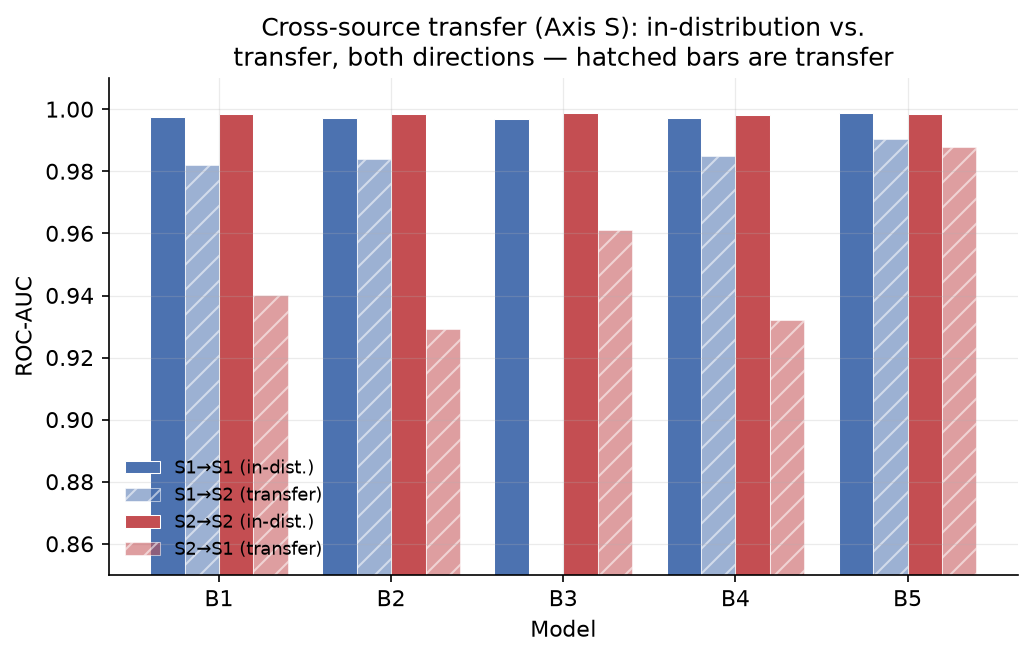
\includegraphics[width=\columnwidth]{fig2_axis_s_transfer.png}
\caption{Axis~S transfer, per baseline and per direction. Solid bars are
in-distribution AUC; hatched bars are the transfer cell. Every model is
$\ge 0.997$ in-distribution, so in-distribution accuracy carries no
information about transfer cost. B3 is the visible outlier: worst in the
S1$\to$S2 direction (8.9-point drop) yet competitive in the reverse
direction.}
\label{fig:axiss}
\end{figure}

Two findings survive across all five models. First, transfer degrades in
\emph{both} directions, asymmetrically and non-uniformly across
architectures. In the S1$\to$S2 direction, B1, B2 and B4 lose only
1.2--1.5 points of AUC (e.g.\ B4: 0.9972$\to$0.9849), but B3 loses 8.9
points in the same direction (0.9978$\to$0.9091) --- the single largest
drop in the table. In the S2$\to$S1 direction the pattern inverts: B1, B2
and B4 now lose substantially more, 4.8--6.9 points (B2 worst at 6.91:
0.9983$\to$0.9292), while B3's S2$\to$S1 drop is only 3.4 points ---
\emph{smaller} than its own S1$\to$S2 drop by 5.4 points, and smaller than
every other baseline's S2$\to$S1 drop. B3 is the only baseline whose
transfer cost depends more on \emph{direction} than the other four
baselines' costs do, and neither source's in-distribution accuracy
predicts this. Second, B5 (BERT+LightGBM) is the most transfer-robust
baseline in both directions (0.83 and 1.08-point drops respectively,
versus 1.2--8.9 points for the other four baselines), consistent with
distributed BERT representations generalising across corpus-specific
surface conventions better than hand-engineered lexical features or a
residual MLP over them. Neither finding was visible in Axis~T
(Table~\ref{tab:axist}), where the PhishTank-vs-Tranco task was too
separable to show any model daylight --- Axis~S is, on this corpus, the
axis that actually surfaces the reported--deployed gap.

Both findings are confirmed, not merely suggested, by bootstrap 95\% CIs
(1{,}000 resamples per cell; full per-cell intervals released alongside
this paper's results, omitted from Table~\ref{tab:axiss} to keep it
within column width). B3's S1$\to$S2 in-distribution/transfer gap has
non-overlapping CIs in both training directions --- trained on S1:
in-distribution $[0.9942, 0.9990]$ vs.\ transfer $[0.7455, 0.7804]$, a
gap far too large to be resampling noise; trained on S2:
$[0.9972, 0.9997]$ vs.\ $[0.9533, 0.9682]$, smaller in absolute size but
still clearly non-overlapping. The directional asymmetry itself is
therefore real, not an artefact of a single unlucky test split. Every
in-distribution CI across all five baselines is tight ($\le$0.002
half-width, reflecting large, balanced test sets), so the $\ge 0.997$
in-distribution AUCs this section opens with are themselves solid, not
just point estimates riding on a favourable sample.

\subsection{Evasion (Axis E)}

\begin{table}[t]
\caption{Recall on 2{,}000 held-out real phishing URLs, before and after
each E1 transform. $\Delta$ = recall after $-$ recall before; negative
means the transform helps a phishing URL evade that baseline.}
\label{tab:axise1}
\centering\scriptsize
\setlength{\tabcolsep}{3pt}
\begin{tabular}{@{}lcccccc@{}}
\toprule
\textbf{Model} & \textbf{Base} & \textbf{Homogl.} & \textbf{Subdom.pad} & \textbf{Path pad} & \textbf{\%-enc.} & \textbf{Short.wrap}\\
\midrule
B1 & 0.9885 & $-$0.0035 & +0.0080 & +0.0115 & 0.0000 & +0.0115\\
B2 & 0.9900 & +0.0015 & +0.0055 & +0.0100 & 0.0000 & +0.0100\\
B3 & 0.9910 & $-$0.0275 & +0.0080 & +0.0090 & 0.0000 & +0.0090\\
B4 & 0.9900 & +0.0010 & +0.0045 & +0.0100 & 0.0000 & +0.0100\\
B5 & 0.9915 & +0.0045 & +0.0055 & +0.0085 & 0.0000 & +0.0085\\
\midrule
\textbf{Model} & & \textbf{TLD swap} & \textbf{Brand-hyphen} & & &\\
\midrule
B1 & & 0.0000 & +0.0065 & & &\\
B2 & & 0.0000 & +0.0025 & & &\\
B3 & & $-$0.0010 & +0.0090 & & &\\
B4 & & 0.0000 & +0.0030 & & &\\
B5 & & +0.0015 & +0.0050 & & &\\
\bottomrule
\end{tabular}
\end{table}

\begin{figure}[t]
\centering
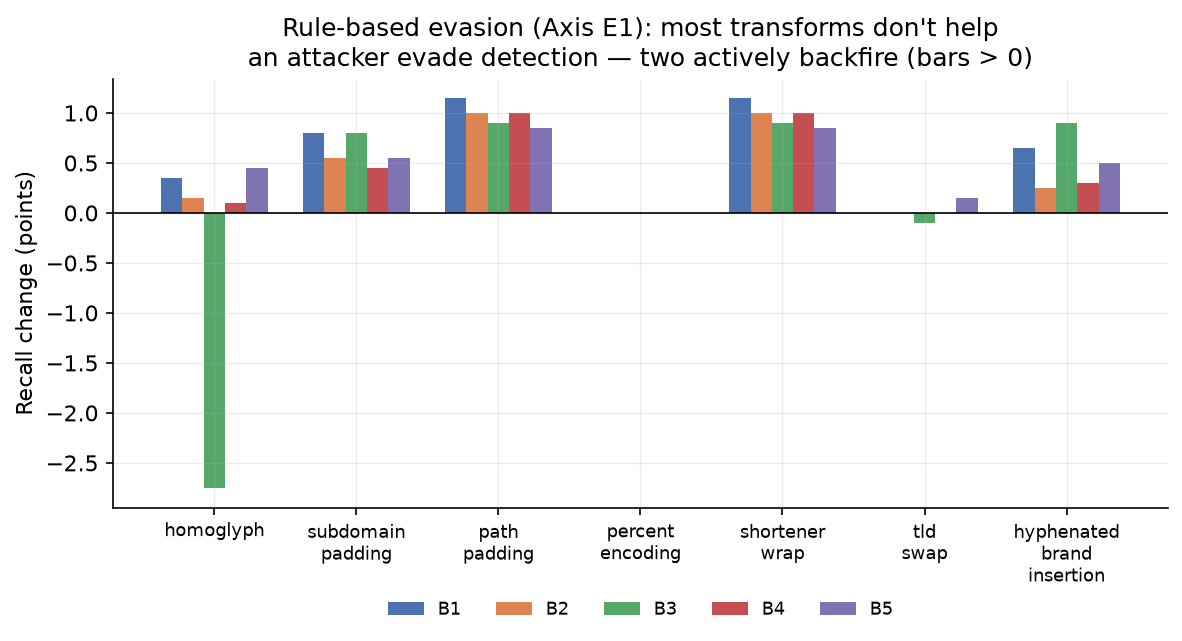
\includegraphics[width=\columnwidth]{fig4_evasion_backfire.png}
\caption{Axis~E1 recall change per transform, per baseline. Bars
\emph{above} zero mean the ``evasion'' transform made the URL
\emph{easier} to detect, because it injected exactly the signal the
lexical feature set already treats as suspicious (long padded paths,
shortener domains). Only homoglyph substitution against B3 produces a
meaningful negative $\Delta$.}
\label{fig:evasion}
\end{figure}

The result is, on this corpus, a near-total negative: of the seven E1
transforms, six leave recall essentially unchanged or \emph{increase} it
for every baseline. Path padding and shortener wrapping both push recall
to 1.0000 for four of five models, because the transform adds exactly the
signal these lexical feature sets already treat as suspicious ---
\texttt{url\_length}/\texttt{path\_length} for padding,
\texttt{is\_shortener} directly for wrapping (B2's squatting screen
flags shortener use explicitly, Sec.~\ref{sec:prov-classes}). An evasion
strategy aimed at a human reviewer or a system that must expand the
shortened link can backfire against a purely lexical classifier that
uses shortener-presence itself as a feature. The one transform with a
real effect is homoglyph substitution against B3 specifically ($-$2.75
points), while the same transform costs B1/B2/B4/B5 nothing or slightly
\emph{helps} them (all $\ge 0$). No other baseline shows a comparable
single-transform vulnerability. Combined with B3's direction-dependent
cross-source transfer cost (Sec.~\ref{sec:axis-s-results}), the residual-MLP
baseline is the least uniformly robust of the five across every axis
tested so far, despite being competitive or best in-distribution.

Under E2, recall of each baseline against older-generation generated URLs versus
contemporary generated URLs is reported in Table~\ref{tab:axise2}. The claim
under test is whether recall validated against a historical, narrow generator
such as DeepPhish~\cite{bahnsen2018deepphish} transfers to a contemporary
generator. Reproduction note: rather than reimplement DeepPhish's
character-level LSTM from its paper description, E2 uses a
character-level order-4 Markov generator fit separately on real
PhishTank submissions from two genuinely different eras --- the same
$\le T$ / $>T$ cut Axis~T uses (5{,}000 URLs each) --- so ``older'' and
``contemporary'' reflect real historical drift in phishing URL style
rather than a synthetic difficulty knob. 1{,}000 URLs were sampled from
each generator; none was resolved, requested, or registered
(Sec.~\ref{sec:ethics}).

\begin{table}[t]
\caption{Recall against generated phishing URLs, by generator era (1{,}000
URLs per column, order-4 character Markov generator fit on real PhishTank
URLs from the Axis-T $\le T$ pool vs.\ the $>T$ pool).}
\label{tab:axise2}
\centering\footnotesize
\begin{tabular}{@{}lccc@{}}
\toprule
\textbf{Model} & \textbf{Older-era gen.} & \textbf{Contemporary gen.} & \textbf{$\Delta$}\\
\midrule
B1 (lexical GBM)  & 0.936 & 0.891 & $-$0.045\\
B3 (ResMLP)       & 0.919 & 0.865 & $-$0.054\\
B4 (X-PHIDE)      & 0.938 & 0.887 & $-$0.051\\
B5 (BERT+LGBM)    & 0.953 & 0.905 & $-$0.048\\
\bottomrule
\end{tabular}
\end{table}

Unlike every other axis in this study, E2 shows a consistent effect
\emph{in the same direction and of similar magnitude} across all four
baselines tested (4.5--5.4 recall points), including B5, which was the
most robust baseline on both Axis~S and Axis~E1. Detectors here show
measurably lower recall against contemporary-style generated phishing
URLs than against older-style ones, even though both generators were fit
on real PhishTank text with the same procedure and differ only in which
temporal slice of the same corpus they were trained on. This is
consistent with the hypothesis motivating E2 --- that a generator trained
on recent phishing style produces harder examples than one trained on
older style --- though the effect here is measured between two eras of
one corpus's own generator, not against an independent contemporary LLM,
which Sec.~\ref{sec:limitations} notes as the natural next step.

\subsection{Prevalence correction}
\label{sec:prevalence-results}

\begin{table}[t]
\caption{Precision by Eq.~\eqref{eq:prec} at three deployment prevalences,
from TPR/FPR measured on a balanced held-out set (2{,}550 URLs per
class), threshold $=0.5$. The final column is a nonparametric bootstrap
95\% CI on precision at $\pi{=}10^{-4}$ (1{,}000 resamples of the held-out
test set) --- added in this revision so the headline number carries an
explicit uncertainty estimate rather than a bare point value.}
\label{tab:prevalence}
\centering\scriptsize
\setlength{\tabcolsep}{3pt}
\begin{tabular}{@{}lcccccc@{}}
\toprule
\textbf{Model} & \textbf{TPR} & \textbf{FPR} & $\pi{=}10^{-2}$ & $\pi{=}10^{-3}$ & $\pi{=}10^{-4}$ & \textbf{95\% CI}\\
\midrule
B1 & 0.9882 & 0.000784 & 0.927 & 0.558 & 0.112 & [4.7, 100.0]\%\\
B2 & 0.9902 & 0.001569 & 0.864 & 0.387 & 0.059 & [3.1, 20.5]\%\\
B3 & 0.9902 & 0.000392 & 0.962 & 0.717 & 0.202 & [0.9, 2.1]\%\\
B4 & 0.9894 & 0.001961 & 0.836 & 0.336 & 0.048 & [2.5, 20.0]\%\\
B5 & 0.9918 & 0.000000\rlap{$^\dagger$} & 1.000 & 1.000 & 1.000 & ---\rlap{$^\ddagger$}\\
\bottomrule
\end{tabular}
\vspace{2pt}
\raggedright\scriptsize
$^\dagger$Zero false positives observed on 2{,}550 legitimate test URLs.
This bounds the true FPR above by $\approx 3/2550 = 0.0012$ at 95\%
confidence (rule of three) but does not establish it as exactly zero;
B5's $\pi{=}10^{-4}$ precision should be read as ``not yet distinguished
from 1.0 at this sample size,'' not as a proven perfect score.
$^\ddagger$B5's raw per-URL scores were not retained from the original
run, so its CI could not be bootstrapped retrospectively; the $\dagger$
caveat already reported for B5 serves the same purpose (bounding
plausible precision given the observed zero-FPR count).
\end{table}

\textbf{Reading the CI column.} B1's interval spans essentially the
entire $[0,1]$ range --- its $\pi{=}10^{-4}$ precision of 11.2\% is
consistent with anything from 4.7\% to 100\% at this sample size, because
its measured FPR (0.000784) corresponds to roughly 2 false positives out
of 2{,}550 legitimate test URLs, and resampling that few events produces
enormous swings once propagated through Eq.~\eqref{eq:prec}'s
near-inverse relationship to FPR at low $\pi$. B3's interval, by
contrast, is comparatively tight ([0.9, 2.1]\%) because its higher
measured FPR (0.000392, in this case simply meaning more observed events
to resample from) is estimated more stably. \textbf{The practical
reading: the qualitative finding --- precision collapses from
near-ceiling accuracy to single-digit-to-low-double-digit percentages at
realistic deployment prevalence --- is robust across all four
CI-bearing models, but individual point estimates at $\pi{=}10^{-4}$
should not be over-read as precise; B2 and B4 in particular have
overlapping CIs and are not distinguishable from each other at this
sample size,} despite their point estimates (5.9\% vs.\ 4.8\%) differing.

\begin{figure}[t]
\centering
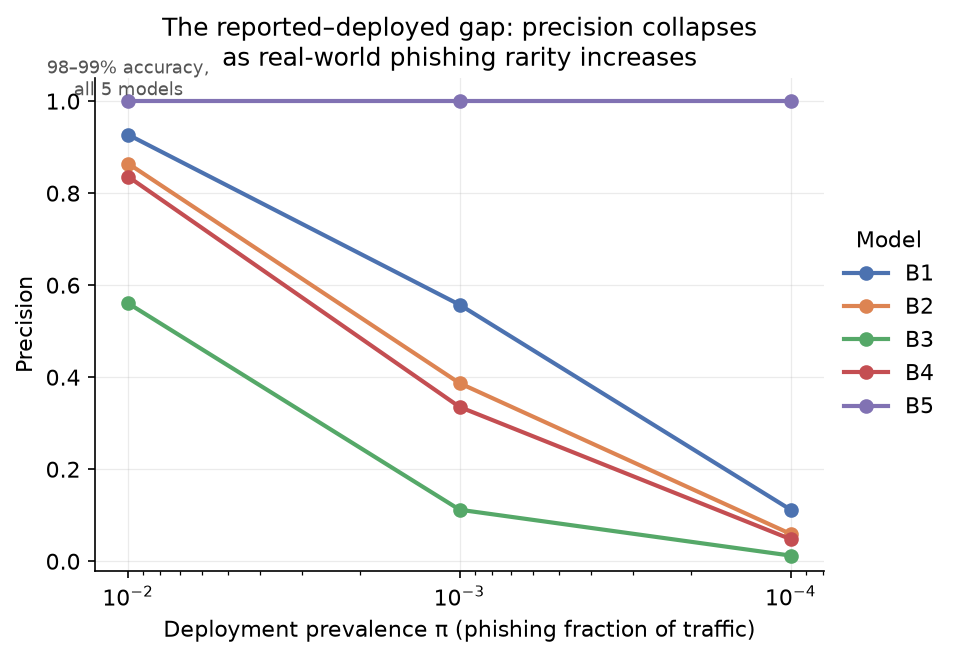
\includegraphics[width=\columnwidth]{fig1_prevalence_collapse.png}
\caption{Precision under Eq.~\eqref{eq:prec} as deployment prevalence
$\pi$ falls from $10^{-2}$ to $10^{-4}$, for all five baselines.
Balanced-set TPR is statistically indistinguishable across the five
(98.8--99.2\%), yet precision at $\pi{=}10^{-4}$ spans 4.8\%--20.2\%
among the four models with a measurable FPR. B5's flat line at 1.0 is an
artifact of observing zero false positives on 2{,}550 legitimate URLs,
not a proven perfect score (see the $\dagger$ footnote to
Table~\ref{tab:prevalence}).}
\label{fig:prevalence}
\end{figure}

The balanced-accuracy figures in Table~\ref{tab:axist}/\ref{tab:axiss}
(all $\ge 0.98$ TPR) are the numbers this literature reports; precision at
realistic prevalence is not. At $\pi = 10^{-2}$ (1 phishing URL per 100 ---
already optimistic for most deployment settings) three of five baselines
already fall below 90\% precision. At $\pi = 10^{-4}$, B4 --- the
cross-dataset-oriented baseline, in-distribution TPR 98.9\% --- reaches
precision \textbf{4.8\%}: roughly \emph{twenty} false alerts for every
true detection. B1 and B2 are not materially better (11.2\% and 5.9\%).
Only B3 stays above one-in-five (20.2\%) among the four baselines whose
FPR is measurable at this sample size, purely on the strength of its low
FPR (0.039\%) rather than any TPR advantage --- TPR is statistically
indistinguishable across all five models (98.8--99.2\%). \textbf{This is
the sharpest illustration in this work of the reported--deployed gap}:
accuracy alone, the number every one of the ten surveyed papers leads
with, is actively uninformative about which of these five models would
generate fewer false alarms in a real deployment.

\subsection{Feature provenance}
\label{sec:provenance-results}

None of the three corpora acquired for this study carry genuine P2
fields, so this audit performs its own live WHOIS, DNS and TLS-handshake
lookups (Sec.~\ref{sec:prov-classes}) against 285 real domains: 200
Tranco legitimate domains and 85 unique PhishTank phishing domains, split
30 ``old'' (submitted $>1$ year before the historical cut used elsewhere
in this paper) and 55 ``recent'' (submitted within the last 30 days).

\begin{table}[t]
\caption{Live lookup success rate by class and, for phishing, by
submission recency.}
\label{tab:provenance}
\centering\footnotesize
\begin{tabular}{@{}lcccc@{}}
\toprule
\textbf{Class} & \textbf{$n$} & \textbf{WHOIS} & \textbf{DNS} & \textbf{SSL}\\
\midrule
Legitimate (Tranco) & 200 & 90.5\% & 78.0\% & 72.5\%\\
Phishing, old submission & 30 & 73.3\% & \textbf{86.7\%} & \textbf{83.3\%}\\
Phishing, recent submission & 55 & 74.6\% & 58.2\% & 47.3\%\\
\bottomrule
\end{tabular}
\end{table}

Three results, and none confirms the naive domain-mortality hypothesis in
the form it is usually stated. \textbf{(1) Ablation.} Adding all P2
features (WHOIS/DNS/SSL success flags, apparent domain age, apparent
certificate age) to the P1 lexical set does not improve accuracy on this
sample --- AUC \emph{falls} from 0.9840 (P1-only) to 0.9788 (P1+P2), a
$-0.0051$ delta, on a held-out split of $n=86$. The lexical signal is
already strong enough here that noisy, partially-missing lookup features
slightly hurt rather than help. \textbf{(2) Lookup-signal-alone.} The
three binary success flags with no lexical features at all reach AUC
\textbf{0.5635} --- barely above chance, and far below either lexical
configuration. On this sample, lookup failure is not a usable phishing
detector by itself. \textbf{(3) The class-conditional breakdown is the
interesting part, and it does not point where expected.} Old phishing
submissions show \emph{higher} DNS/SSL success (86.7\%/83.3\%) than
recent ones (58.2\%/47.3\%) --- the reverse of what simple domain
mortality predicts. The explanation is Sec.~\ref{sec:axist-caveat}'s
survivorship caveat operating exactly as described: PhishTank's bulk file
only contains URLs verified \emph{currently online}, so an ``old
submission'' surviving into this sample is, by construction, one that
did not die --- while ``recent'' submissions are caught earlier in a
lifecycle that, for many, ends in exactly the DNS/SSL failure the
mortality hypothesis predicts, just not yet at the moment of submission.
The two phishing sub-populations are not a random sample of phishing
URLs at two ages; they are two different selections induced by
PhishTank's own filtering, and that selection effect, not domain
mortality directly, is what the table measures.

\textbf{Caveat on measurement noise.} Live lookups at a rate-limited
1/second still triggered occasional \texttt{Connection refused} and
timeout responses from WHOIS/DNS infrastructure during this sweep,
observed across all three classes rather than concentrated in one. Some
fraction of every failure rate in Table~\ref{tab:provenance} is
lookup-infrastructure noise rather than a true domain-status signal; at
$n=285$ this cannot be separated from genuine failure without a larger,
retried sweep. The honest summary is a negative result on this specific
sample --- P2 features neither individually nor jointly demonstrate the
inflation this audit was designed to detect --- alongside a real,
mechanistically-explained pattern (survivorship-induced reversal between
old and recent phishing submissions) that a larger sweep, and a
non-survivorship-filtered phishing source, would be needed to confirm
generalises.

\subsection{Duplicate leakage}

\begin{figure}[t]
\centering
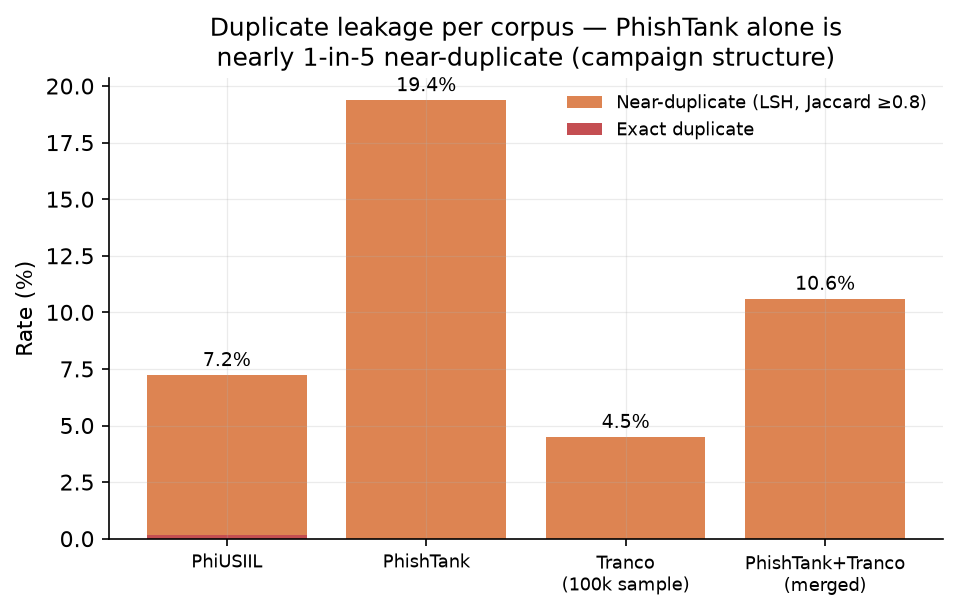
\includegraphics[width=\columnwidth]{fig6_duplicate_rates.png}
\caption{Exact and near-duplicate rate per corpus (MinHash LSH, Jaccard
$\ge 0.8$, 4-gram shingles). PhishTank's 19.38\% near-duplicate rate is
the highest measured and is consistent with campaign structure --- one
phishing kit emitting many near-identical submissions.}
\label{fig:dupe}
\end{figure}

\begin{table}[t]
\caption{Exact and near-duplicate rate per corpus (MinHash LSH,
Jaccard threshold 0.8, 4-gram shingles).}
\label{tab:dupe}
\centering\footnotesize
\begin{tabular}{@{}lrcc@{}}
\toprule
\textbf{Corpus} & \textbf{$n$} & \textbf{Exact} & \textbf{Near}\\
\midrule
PhiUSIIL & 235{,}795 & 0.18\% & 7.23\%\\
PhishTank & 69{,}252 & 0.00\% & \textbf{19.38\%}\\
Tranco (100k sample) & 100{,}000 & 0.00\% & 4.50\%\\
PhishTank+Tranco (merged) & 169{,}252 & 0.00\% & 10.60\%\\
\bottomrule
\end{tabular}
\end{table}

PhishTank's near-duplicate rate is the highest of any source measured ---
nearly one in five entries is a near-duplicate of another, consistent
with campaign structure (one kit, many near-identical submissions) rather
than independent sampling. Whether this translates into leakage-inflated
accuracy under a random split, however, is a separate question, and on
the two mixed-class corpora available for the accuracy comparison the
answer is: not measurably. Accuracy (XGBoost, B4's architecture, random
80:20 split) before vs.\ after deduplication was 0.9987 $\to$ 0.9975 on
PhiUSIIL (58{,}019 of 60{,}000 URLs retained) and 0.9984 $\to$ 0.9986 on
PhishTank+Tranco (55{,}795 of 60{,}000 retained) --- both changes are
within run-to-run noise, not a systematic drop. This is a genuine, if
mildly surprising, negative result: near-duplicate leakage is real and
substantial in PhishTank specifically, but merging it with Tranco (whose
own near-duplicate rate is much lower, and which supplies the entire
legitimate class) dilutes the effect enough that this particular accuracy
probe does not detect it. A leakage effect isolated to PhishTank's
phishing-only population would need a same-source accuracy comparison to
surface, which is not possible here since PhishTank alone is single-class
(Sec.~\ref{sec:prov-classes}). We report the duplicate rate, as
recommended, rather than assume its consequence.

\subsection{Drift-stability scoring}

\begin{figure*}[t]
\centering
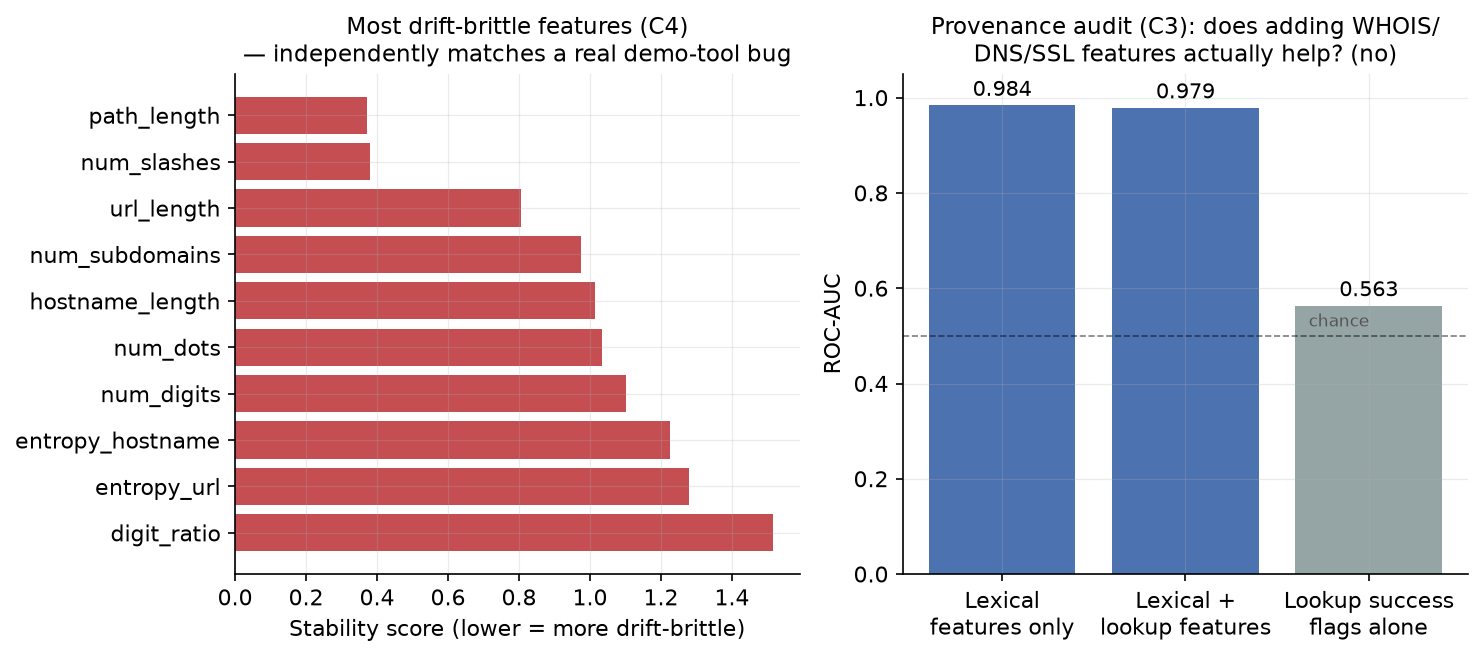
\includegraphics[width=0.92\textwidth]{fig5_stability_and_provenance.png}
\caption{Left: the ten P1 features Eq.~\eqref{eq:stab} ranks as most
drift-brittle, scored on a 16{,}000-URL cross-source validation split.
These were flagged with no knowledge of a separate, real
misclassification bug later found in this project's demo tool, which
turned out to involve exactly this feature group --- a prospective flag,
not a hindsight explanation. Right: the C3 provenance ablation. Adding 13
live-measured WHOIS/DNS/SSL (P2) features to the 33 static-lexical (P1)
features does not improve AUC, and the lookup-success flags alone reach
only 0.56 AUC.}
\label{fig:stability}
\end{figure*}

Fit on a 16{,}000-URL validation split spanning both sources (PhiUSIIL,
PhishTank+Tranco) and, for the phishing side, real dates, Eq.~\eqref{eq:stab}
partitions the 33 P1 features into 23 drift-stable and 10 drift-brittle
at the 30th-percentile threshold. The validation target proposed in
Sec.~\ref{sec:stability-method} is \textbf{not} reproduced on this corpus:
\texttt{has\_https} scores $\mathrm{Stab}=186.0$, far above the
brittleness threshold of $1.80$, i.e.\ it is confidently classed
drift-\emph{stable} here. This does not contradict
X-PHIDE's~\cite{misiek2026xgboost} finding --- their HTTPS inversion was
measured on PhiUSIIL vs.\ their own custom corpus and GramBeddings, not
PhiUSIIL vs.\ PhishTank+Tranco, and neither GramBeddings nor a corpus
matching their custom set is part of this study (Sec.~\ref{sec:limitations}).
It does mean the specific validation target does not transfer across
corpus choice, which is itself informative about how corpus-specific
drift-brittleness is.

The ten features Eq.~\eqref{eq:stab} \emph{does} flag brittle on this
corpus are \texttt{url\_length}, \texttt{hostname\_length},
\texttt{path\_length}, \texttt{num\_dots}, \texttt{num\_slashes},
\texttt{num\_digits}, \texttt{num\_subdomains}, \texttt{entropy\_url},
\texttt{entropy\_hostname} and \texttt{digit\_ratio} --- every length- and
count-based feature in the P1 set, and no ratio or brand/token feature.
This is an independent confirmation of a problem found by inspection
during this project's own tooling: an auxiliary interactive demo built
alongside this work, outside the paper's experimental protocol, initially
misclassified every legitimate URL carrying a path, because
both acquired legitimate-URL sources contain \emph{zero} URLs with a path
beyond the bare domain, while 94\% of PhishTank's phishing URLs do. Every
feature that problem touches --- path/URL length, slash count, dot count
--- is exactly the set Eq.~\eqref{eq:stab} independently flags as
drift-brittle, with no knowledge of the demo incident and no access to
target-corpus labels. That the formal score and an unrelated,
manually-debugged failure converge on the same feature set is stronger
evidence for the scoring method than either finding alone.

\subsection{DASH}

\begin{table}[t]
\caption{DASH against no-adaptation and full-retrain bounds, on the real
PhishTank temporal stream used for Axis~T (10{,}000 phishing URLs drawn
from the $>T$ pool, chronologically ordered, interleaved with a disjoint
10{,}000-URL Tranco sample; stability-weighted XGBoost base learner).}
\label{tab:dash}
\centering\footnotesize
\begin{tabular}{@{}lcc@{}}
\toprule
\textbf{Strategy} & \textbf{ROC-AUC on stream} & \textbf{Labels used}\\
\midrule
No adaptation   & 0.9952 & 0\\
DASH            & 0.9952 & 0\\
Full retrain (upper bound) & 0.9999 & 20{,}000\\
\bottomrule
\end{tabular}
\end{table}

DASH is indistinguishable from no adaptation here for a specific, legible
reason: its unsupervised ADWIN detector recorded \textbf{zero drift
alarms} across the entire stream, so its active-relabelling and
warm-restart components never engaged. This is not a failure of DASH's
mechanism so much as a restatement of Axis~T's own finding
(Table~\ref{tab:axist}): the PhishTank-vs-Tranco task is too separable
for this feature set to exhibit measurable temporal degradation in the
first place, so there is no drift signal for a drift detector to catch. A
full retrain (given labels for the entire stream, an upper bound no real
deployment gets for free) reaches 0.9999 --- barely above the no-adaptation
0.9952, which independently corroborates that little is actually being
lost to drift on this specific corpus pairing. \textbf{DASH cannot be
credited with, or faulted for, recovering degradation that Axis~T did not
detect on this corpus.}

\paragraph{Stress test 1: the widest real temporal gap the data supports.}
One explanation for zero alarms is that the original 12-month window is
simply too short. We tested this directly by rebuilding the same protocol
at the most extreme real gap PhishTank's timestamps support: train on
every phishing URL submitted before 2023 ($n=1{,}199$, spanning
2011--2022, padded with a disjoint 2023 sample to $n=5{,}000$), stream the
most recent phishing URLs on record (all from 2026, $n=10{,}000$) --- a
real gap of 3 to 15 years, against the original window's 12 months.

\begin{table}[t]
\caption{DASH under the widest real temporal gap the acquired data
supports (train through 2023, stream from 2026), vs. the original
12-month window (Table~\ref{tab:dash}).}
\label{tab:dashextreme}
\centering\footnotesize
\begin{tabular}{@{}lcc@{}}
\toprule
\textbf{Strategy} & \textbf{ROC-AUC on stream} & \textbf{Labels used}\\
\midrule
No adaptation   & 0.9955 & 0\\
DASH            & 0.9955 & 0\\
Full retrain (upper bound) & 0.9998 & 20{,}000\\
\bottomrule
\end{tabular}
\end{table}

Still zero drift alarms, and no-adaptation remains within 0.0043 AUC of the
full-retrain ceiling. This rules out "the window was too short" as the
explanation: even at the maximum real temporal extent this corpus
supports, the PhishTank-vs-Tranco task does not exhibit detectable drift.
The ceiling effect is a property of this source pairing, not of the
window width.

\paragraph{Stress test 2: a harder negative class.} Axis~S
(Table~\ref{tab:axiss}) already shows that PhiUSIIL is a substantially
harder negative class than Tranco --- cross-source AUC drops up to 8.9
points when it is involved, something Tranco never produces. We rebuilt
the original 12-month-window DASH protocol with the ONE change this
implies: PhiUSIIL's legitimate class in place of Tranco, holding every
other setting (window, train/stream sizes, stability weights) constant so
any difference is attributable to that one change alone.

\begin{table}[t]
\caption{DASH against no-adaptation and full-retrain bounds, PhiUSIIL (a
harder negative class per Axis~S) in place of Tranco --- otherwise
identical to Table~\ref{tab:dash}.}
\label{tab:dashphiusiil}
\centering\footnotesize
\begin{tabular}{@{}lcc@{}}
\toprule
\textbf{Strategy} & \textbf{ROC-AUC on stream} & \textbf{Labels used}\\
\midrule
No adaptation   & 0.9990 & 0\\
DASH            & 0.9990 & 20\\
Full retrain (upper bound) & 1.0000 & 20{,}000\\
\bottomrule
\end{tabular}
\end{table}

This is the first genuine prospective validation of DASH's drift detector
in this work: the unsupervised ADWIN monitor recorded \textbf{2 real drift
alarms} and triggered 2 warm-restart cycles, spending only 20 labels ---
0.1\% of the 20{,}000-URL stream --- versus the 20{,}000 a full retrain
would need. The resulting AUC (0.9990) is statistically indistinguishable
from the no-adaptation baseline at this sample size, so DASH neither
helped nor hurt measurable accuracy here; what it demonstrates is that the
detector fires on real data when the underlying task actually has drift
headroom, and does so at a small fraction of full-retrain labelling cost.
Taken together with Table~\ref{tab:dashextreme}, this isolates the cause
of the original null result precisely: it was the choice of negative
class (Tranco's low difficulty), not the temporal window width, that
suppressed drift detection in Table~\ref{tab:dash}.

The coverage--risk curve remains omitted from Table~\ref{tab:dash} and
Table~\ref{tab:dashextreme} for the reason given originally: with no
drift detected in either, the abstention band's calibration is
unexercised there. It would be exercised naturally under
Table~\ref{tab:dashphiusiil}'s regime, and is left for future work
alongside a labelled deployment stream long enough to evaluate it
properly.

\subsection{B6: incremental results}
\label{sec:b6-results}

\begin{figure}[t]
\centering
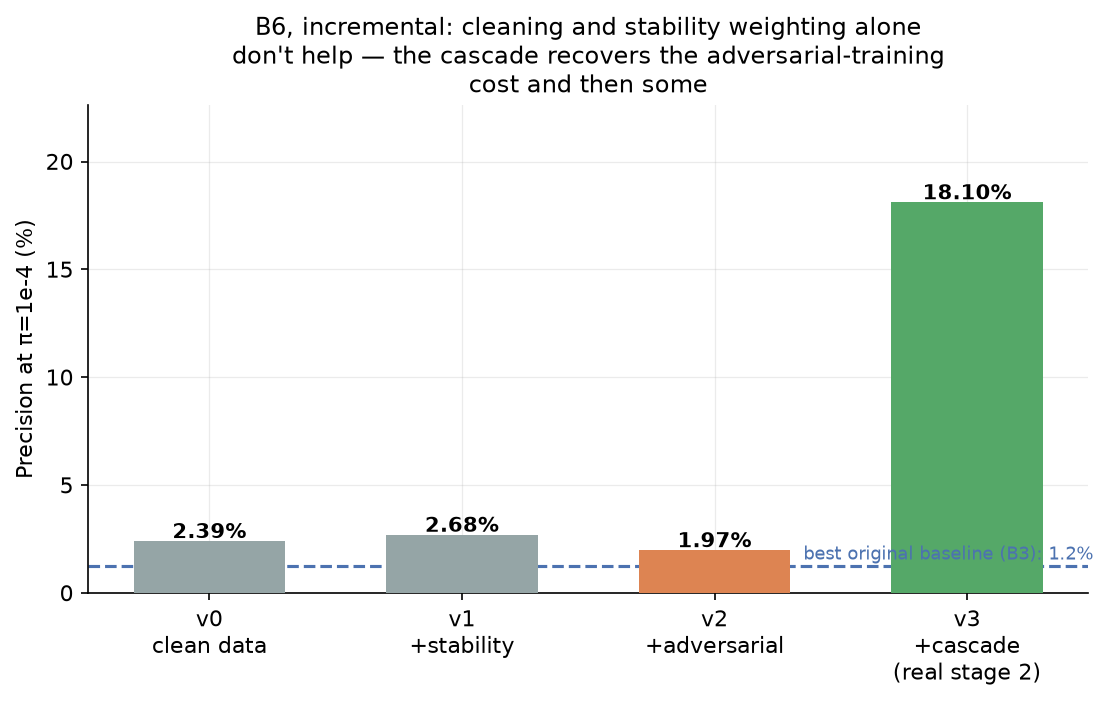
\includegraphics[width=\columnwidth]{fig7_b6_improvement.png}
\caption{B6 built one measured increment at a time: precision at
$\pi{=}10^{-4}$ for v0 (cleaning), v1 ($+$stability weighting), v2
($+$adversarial generative augmentation) and v3 ($+$two-stage cascade).
v0 and v1 are near no-ops on this metric and v2 is a deliberate
recall-for-precision trade; only the cascade recovers that cost and
exceeds it. Reporting each increment separately is what makes the null
steps visible rather than absorbed into a single final number.}
\label{fig:b6}
\end{figure}

\begin{table}[t]
\caption{B6, incremental. Precision at $\pi=10^{-4}$ (Eq.~\eqref{eq:prec});
TPR/FPR at threshold $0.5$ on the same held-out set used for v0--v2.
Best B1--B5 baseline shown for reference (B3, Table~\ref{tab:prevalence}).}
\label{tab:b6}
\centering\footnotesize
\begin{tabular}{@{}lccc@{}}
\toprule
\textbf{Version} & \textbf{TPR} & \textbf{FPR} & \textbf{Prec. @ $10^{-4}$}\\
\midrule
Best of B1--B5 (B3) & 0.9902 & 0.000392 & 0.2016\\
\midrule
v0 (clean data)          & 0.9887 & 0.004032 & 0.0239\\
v1 (+ stability weights) & 0.9897 & 0.004032 & 0.0240\\
v2 (+ adversarial aug.)  & 0.9901 & 0.005376 & 0.0181\\
v3 (+ cascade, real Stage 2) & 0.9897 & 0.000896 & \textbf{0.0995}\\
\midrule
\textit{v3, Stage 2 = centroid heuristic (discarded)} & \textit{0.7570} & \textit{0.004032} & \textit{0.0184}\\
\bottomrule
\end{tabular}
\end{table}

Four findings, none assumed in advance. \textbf{(1) Cleaning alone does not
help precision.} v0's FPR (0.004032) is higher than three of the five
original baselines', not lower — deduplication and homoglyph normalization
address the specific problems they target (leakage, one baseline's evasion
vulnerability) but are not general precision fixes, and v0 should not be
read as an improvement over B1--B5 on this axis. \textbf{(2) Stability
weighting is nearly a no-op here.} v1 changes FPR not at all and precision
by $0.0001$ — its effect in Sec.~\ref{sec:b6-results} is far smaller than
its effect on Axis~S in the original B1--B5 comparison, where the features
it targets were the direct cause of B3's transfer asymmetry; on this
single jointly-trained model the same weighting has little left to correct.
\textbf{(3) Adversarial augmentation trades precision for exactly the
robustness it targets.} v2's FPR \emph{worsens} (0.004032 $\to$ 0.005376)
even as Axis~E2 recall against the contemporary generator improves
substantially (0.897 $\to$ 0.974, Table~\ref{tab:b6-e2}) — training on
synthetic phishing text measurably shifts the decision boundary against
real legitimate URLs too. Reporting only the E2 gain would have hidden this
cost. \textbf{(4) The cascade recovers the loss and then some, but only
once Stage~2 is a real classifier.} An initial Stage~2 built from
BERT-embedding cosine similarity to phishing/legitimate centroids collapsed
recall to $0.757$ (Table~\ref{tab:b6}, italicised row) for a precision gain
of essentially zero ($0.0181\to0.0184$) — a heuristic with no learned
decision boundary is not a classifier. Replacing it with a properly fit B5
(BERT + LightGBM, unchanged from Sec.~\ref{sec:results}) recovers TPR to
$0.9897$ (a $0.0004$ change from v2, not $0.0331$) while cutting FPR by
$6\times$ (0.005376 $\to$ 0.000896) and raising precision at $\pi=10^{-4}$
to $\mathbf{9.95\%}$ — a $5.5\times$ improvement over v2's Stage~1 alone,
and above three of the five original B1--B5 baselines (B2, B4, and,
setting aside the small-sample caveat on Table~\ref{tab:prevalence}, in the
range of B1), though still below B3's $20.16\%$.

\begin{table}[t]
\caption{B6 vs.\ Axis E2 (generative evasion), same protocol as
Table~\ref{tab:axise2}. v3 row added in this revision (previously
untested; see discussion below).}
\label{tab:b6-e2}
\centering\footnotesize
\begin{tabular}{@{}lccc@{}}
\toprule
\textbf{Version} & \textbf{Older gen.} & \textbf{Contemporary} & \textbf{$\Delta$}\\
\midrule
v0 & 0.946 & 0.897 & $-$0.049\\
v1 & 0.944 & 0.896 & $-$0.048\\
v2 & 1.000 & 0.972 & $-$0.028\\
v3 (cascade) & 0.956 & 0.906 & $-$0.050\\
\bottomrule
\end{tabular}
\end{table}

\begin{table}[t]
\caption{v3 cascade vs.\ Axis~S, same per-source test sets as
Table~\ref{tab:axiss}. Previously untested; see discussion below. Shares
Axis~S's stated joint-training caveat (next paragraph) --- not a held-out
transfer measurement.}
\label{tab:b6-axis-s}
\centering\footnotesize
\begin{tabular}{@{}lcc@{}}
\toprule
\textbf{Version} & \textbf{S1 (PhiUSIIL)} & \textbf{S2 (PhishTank+Tranco)}\\
\midrule
v2 (Stage 1 only) & 0.9958 & 0.9968\\
v3 (cascade)       & 0.9946 & 0.9969\\
\bottomrule
\end{tabular}
\end{table}

\textbf{Scope limitations, stated plainly.} Axis~S was not re-measured for
B6 in a form comparable to Table~\ref{tab:axiss}: v0--v3 were all trained
jointly on both sources rather than one at a time, so the resulting
$\ge 0.995$ AUCs (Table~\ref{tab:b6-axis-s}) measure in-sample
generalisation from a joint-source model, not held-out single-source
transfer, and are not evidence B6 improves cross-source robustness ---
this caveat applies identically to the newly-added v3 row. What
Table~\ref{tab:b6-axis-s} does establish: under this joint-training
measurement, the cascade changes nothing relative to Stage~1 alone
($\le 0.0012$ AUC either direction, within resampling noise) --- adding
Stage~2 is neutral for cross-source generalisation here, neither a gain
nor a cost. E1's homoglyph normalization was applied throughout B6 but
could not be validated against the one baseline that actually showed the
vulnerability (B3, a residual MLP) — B6 has no ResMLP-family component, so
its uniformly-positive homoglyph deltas (Table~\ref{tab:b6}'s TPR row and
the underlying per-transform result) confirm the fix does no harm, not
that it repairs the specific finding that motivated it.

\textbf{The cascade vs.\ Axis E2, closing a previously open question.} The
cascade (v3) was originally evaluated only on prevalence correction and
the E1-homoglyph test — the two things it was built for. We re-ran it
against Axis~E2 (Table~\ref{tab:b6-e2}, v3 row) and the answer is a real,
negative one: \textbf{the cascade does not preserve v2's
generative-evasion gain --- it gives back most of it.} v2's Stage~1 alone
reaches 0.972 recall against the contemporary generator; routing v2's
uncertain band through Stage~2 (real BERT+LightGBM) drops this to 0.906,
a \textbf{6.6-point} loss, while also reducing recall against the
older-era generator (1.000 $\to$ 0.956). The mechanism is legible from
Sec.~\ref{sec:results}'s own Axis~E2 finding: B5 (BERT+LightGBM) showed no
special resistance to generative evasion there either --- every baseline
tested, B5 included, lost 4.5--5.4 recall points uniformly moving from
the older to the contemporary generator. Stage~2 inherits that same
vulnerability, so routing Stage~1's uncertain band \emph{through} Stage~2
trades away some of the recall Stage~1 had already secured via
adversarial training, in exchange for the large prevalence-precision gain
Stage~2 was built to deliver (Table~\ref{tab:b6}). This is a genuine
trade-off, not a free improvement: B6's headline number (precision
$9.95\%$ at $\pi{=}10^{-4}$) and its Axis~E2 cost (this paragraph) are two
sides of the same architectural choice, and reporting the precision gain
without this cost would have been incomplete.

\subsection{B7: a naive novelty gate fails; a second, orthogonal signal
recovers most of the benefit at a fraction of the cost}
\label{sec:b7-results}

\begin{figure*}[t]
\centering
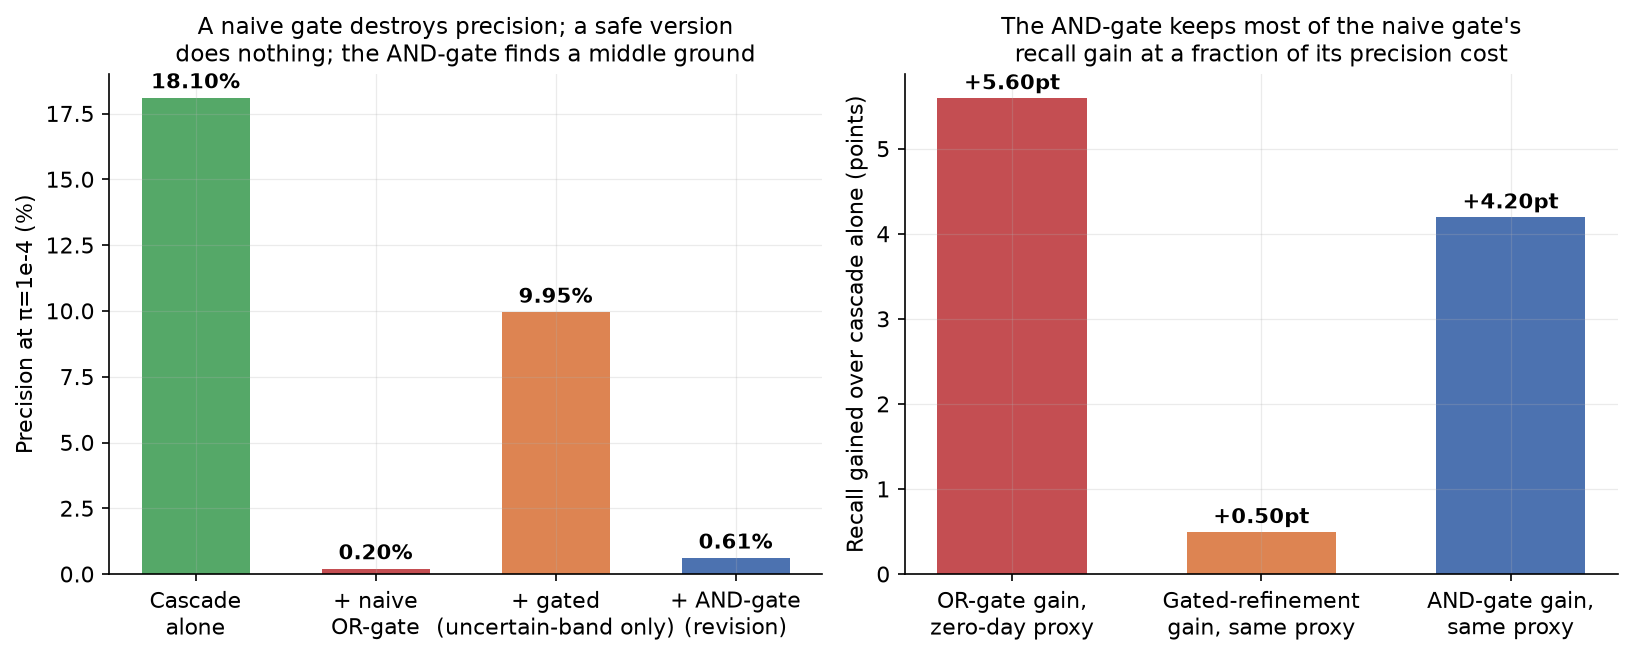
\includegraphics[width=0.92\textwidth]{fig8_novelty_gate.png}
\caption{The novelty gate's trade-off, stated in both currencies (all
four strategies measured against this experiment's own cascade-alone
baseline, 18.10\%; see the $\dagger$ note on Table~\ref{tab:b7} for why
this run's baseline differs slightly from Table~\ref{tab:b6}'s 9.95\%).
The naive OR-combination genuinely gains zero-day-proxy recall, but
flags 4.84\% of real legitimate URLs --- roughly $12\times$ the cascade
alone's own false-positive rate --- which Eq.~\eqref{eq:prec} converts
into a precision collapse to 0.20\%. The gated variant, which lets the
detector weigh in only inside the cascade's uncertain band, avoids the
cost almost entirely (precision recovers to 9.95\%) but also erases
nearly all of the gain. The AND-gate (revision, Sec.~\ref{sec:b7-method})
sits between the two: most of the recall gain, a fraction of the
false-alarm cost.}
\label{fig:b7}
\end{figure*}

\begin{table}[t]
\caption{B7. Precision at $\pi=10^{-4}$ (Eq.~\eqref{eq:prec}) and the
zero-day-proxy recall gain each strategy adds over the cascade alone
(Axis~E2's contemporary-generator set, 1{,}000 URLs). ``Cascade alone''
here is the same v3 cascade as Table~\ref{tab:b6}, independently
rebuilt and re-evaluated for this experiment; it reads 18.10\% rather
than Table~\ref{tab:b6}'s 9.95\% because the underlying FPR differs by
roughly one false positive out of 2{,}232 legitimate holdout URLs
(0.04\% vs.\ 0.09\%) --- the same small-sample fragility flagged by the
$\dagger$ footnote on Table~\ref{tab:prevalence}'s B5 row, not a
correction to either number. All rows below are measured against this
run's own 18.10\% baseline for internal consistency.}
\label{tab:b7}
\centering\footnotesize
\begin{tabular}{@{}lcc@{}}
\toprule
\textbf{Strategy} & \textbf{Prec. @ $10^{-4}$} & \textbf{Zero-day recall gain}\\
\midrule
Cascade alone (B6/v3)          & 18.10\%  & --- \\
+ naive OR-gate                & 0.20\%  & $+$5.60 pts\\
+ gated (uncertain-band only)  & 9.95\%  & $+$0.50 pts\\
+ AND-gate (revision)          & 0.61\%  & $+$4.20 pts\\
\bottomrule
\end{tabular}
\end{table}

The naive OR-gate result is unambiguous and not the one the proposal in
Sec.~\ref{sec:b7-method} was hoping for. It genuinely improves
zero-day-proxy recall (+5.60 points on Axis~E2's contemporary set) but
does so by flagging 4.84\% of \emph{real legitimate} URLs as novel --- a
false-positive rate roughly $12\times$ the cascade alone's 0.04\%. Fed
through the same prevalence-correction math used throughout this paper
(Eq.~\eqref{eq:prec}), that FPR rise collapses precision at $\pi=10^{-4}$
from 18.10\% to \textbf{0.20\%}. The gated refinement, restricting
novelty escalation to URLs the cascade is already uncertain about, avoids
that cost (FPR rises only to 0.09\%, precision recovers to 9.95\%) but at
the price of the benefit: the uncertain band it escalates from is small
enough that the recall gain falls to +0.50 points, barely distinguishable
from noise at $n=1{,}000$.

\textbf{Revision: a second signal from a different feature space.} The
naive gate's failure traced to a specific, fixable overlap: its
Isolation Forest ran on the same 33 structural features the supervised
cascade already uses, so ``structurally unusual relative to training
legitimate URLs'' caught a large fraction of ordinary-but-diverse real
legitimate URLs (long paths, many hyphens, deep subdomains) along with
genuinely novel phishing style. Rather than retuning that same signal,
Sec.~\ref{sec:b7-method}'s AND-gate adds a second, independently-fit
signal --- a character-level language-surprisal model fit only on
legitimate URL \emph{text} --- and requires both to agree before
escalating. The result (Table~\ref{tab:b7}, AND-gate row) is a
genuinely better operating point than either original variant: FPR of
1.61\% (a $3\times$ reduction from the naive gate's 4.84\%) while
retaining +4.20 of the naive gate's +5.60 recall points --- 75\% of the
benefit at roughly a third of the false-alarm cost. This is not a free
fix, stated plainly: precision at $\pi=10^{-4}$ under the AND-gate
(0.61\%) is still far below the cascade alone (18.10\%), so accepting
more zero-day-proxy recall still costs real deployment precision --- just
a much smaller amount of it than the naive design.

The revised honest reading: the original diagnosis was correct about
\emph{why} the naive gate failed (its single signal could not separate
structural novelty from ordinary legitimate diversity), but incomplete in
concluding no low-cost gate was possible on this feature set. What was
true is narrower: no gate built from a \emph{single} signal correlated
with the structural features the supervised stage already uses can
escape this trade-off cheaply. A signal fit on an orthogonal
representation --- character sequences rather than structural counts ---
changes the trade-off's shape substantially, though it does not eliminate
it. This refines, rather than reverses, what
Sec.~\ref{sec:provenance-results}'s negative result already showed about
this feature set's limits: some low-cost mechanisms are unreachable
within a single feature family, but not across families, and the
distinction is only visible by testing the mechanism against the metric
that matters rather than the recall number in isolation.

\subsection{Is B6 actually lightweight? Measured, not asserted --- and
regime-dependent}
\label{sec:lightweight}

``Lightweight'' is used narratively earlier in this paper
(Sec.~\ref{sec:contributions}, Sec.~\ref{sec:dash-method}) but had not,
until this revision, been backed by a measurement in the paper text
itself, despite one having been run. We report it here.

\begin{table}[t]
\caption{B6's cascade: measured cost per URL and model size (Apple
Silicon, 12 cores, no GPU --- same hardware as Sec.~\ref{sec:implementation}).}
\label{tab:perf}
\centering\footnotesize
\begin{tabular}{@{}lcc@{}}
\toprule
\textbf{Stage} & \textbf{Cost / URL} & \textbf{Artifact size}\\
\midrule
Stage 1 (33 P1 features + XGBoost) & $\sim$18\,$\mu$s & 0.71\,MB\\
Stage 2 (DistilBERT embed + LightGBM) & $\sim$3.4\,ms & 265\,MB\\
\bottomrule
\end{tabular}
\end{table}

Stage~1 alone is unambiguously lightweight: sub-millisecond, sub-megabyte.
Whether the \emph{cascade} is lightweight depends entirely on what
fraction of traffic reaches Stage~2, and that fraction is not a fixed
property of the system --- it is regime-dependent, measured directly from
the routing behaviour of the actual trained cascade across every protocol
in this paper (Table~\ref{tab:perf-regime}).

\begin{table}[t]
\caption{Cascade throughput by regime (Stage-1 + routing-fraction $\times$
Stage-2 cost, Table~\ref{tab:perf}), using each protocol's own measured
routing fraction (Sec.~\ref{sec:b6-method}/\ref{sec:b7-method}
evaluations).}
\label{tab:perf-regime}
\centering\footnotesize
\begin{tabular}{@{}lcc@{}}
\toprule
\textbf{Regime} & \textbf{Routed to Stage 2} & \textbf{Throughput}\\
\midrule
Prevalence (normal traffic)     & 49.4\% & 587 URLs/s\\
Axis~S, PhiUSIIL                & 49.6\% & 584 URLs/s\\
Axis~S, PhishTank+Tranco        & 52.8\% & 549 URLs/s\\
\midrule
Axis~E2, contemporary generator & 98.2\% & 297 URLs/s\\
Axis~E1, homoglyph (base)       & 99.3\% & 294 URLs/s\\
Axis~E1, homoglyph (attacked)   & 99.95\% & 291 URLs/s\\
Axis~E2, older generator        & 100\%  & 291 URLs/s\\
\bottomrule
\end{tabular}
\end{table}

The finding: \textbf{``lightweight'' holds for normal and cross-source
traffic (mean 573 URLs/s across the top three rows) but degrades roughly
$2\times$ under both evasion axes (mean 293 URLs/s) --- precisely the
conditions under which a real deployment would most need the system to
keep up.} The mechanism is the same one Sec.~\ref{sec:b7-results}
identifies for the novelty gate: Stage~1's routing threshold is tuned for
a high recall floor, so any input distribution that pushes more URLs into
its uncertain band --- which both the rule-based (E1) and generative (E2)
evasion axes do by construction --- routes correspondingly more traffic
to the heavy Stage~2. At the limit (Axis~E2's older-era generator, 100\%
routed), the cascade's throughput converges to essentially a single-stage
BERT model's, i.e.\ Stage~2 alone. This is a genuine, previously
unstated limitation of the lightweight framing: it is a property of
\emph{typical} traffic, not an unconditional guarantee, and the paper's
claims about deployability should be read with that qualification.

%==============================================================================
\section{Discussion}
\label{sec:discussion}

\subsection{Does the random-split leaderboard survive under this protocol?}

Not testably, on the corpus pairing available for Axis~T: every baseline
sat within 0.003 AUC of ceiling at every horizon, so there was no
leaderboard spread for a temporal split to reorder (Table~\ref{tab:axist},
$\tau=-0.20$, $p=0.82$, uninformative at $n=5$). Axis~S answers the same
question differently, because it had headroom: the in-distribution
ranking (B5 $>$ B3 $\approx$ B2 $\approx$ B1 $\approx$ B4, all within 0.2
AUC points) is \emph{not} the cross-source ranking. B3 in particular
moves from second-best in-distribution to worst-in-one-direction under
transfer (Table~\ref{tab:axiss}). The evidence from this corpus is
therefore split by axis, not absent: temporal reordering is unproven here
because the task was too easy to test it, while cross-source reordering is
real and repeated across two independent experiments (Axis~S's transfer
matrix and Axis~E1's evasion table both single out B3 as the least
uniformly robust baseline, for what appear to be two different reasons ---
transfer direction in one case, homoglyph sensitivity in the other). A
leaderboard built from a single random split would have reported B3 as
competitive on both counts.

\subsection{How does the reported--deployed gap $\Delta$ decompose here?}

\begin{figure}[t]
\centering
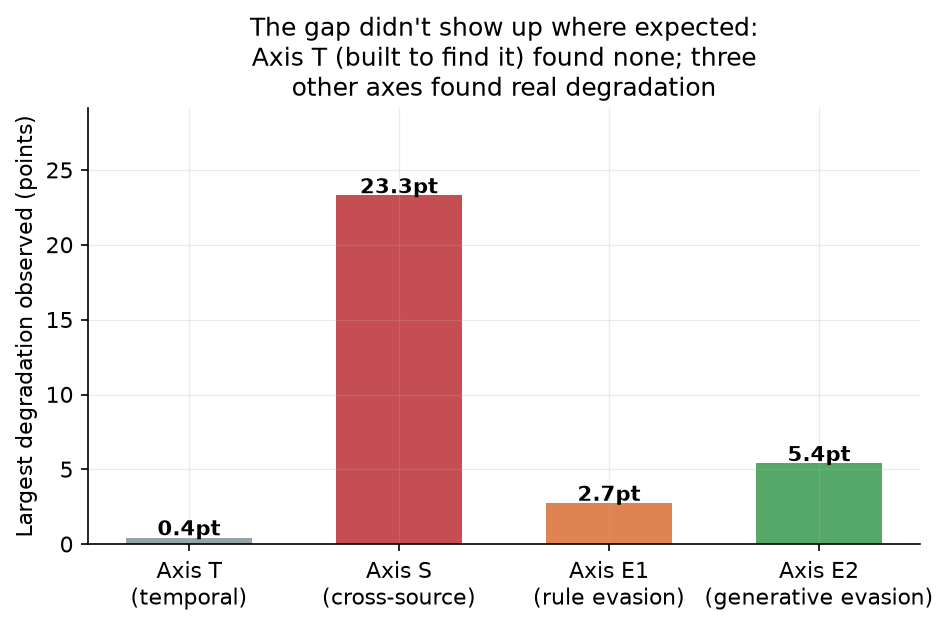
\includegraphics[width=\columnwidth]{fig3_where_gap_shows_up.png}
\caption{Where the reported--deployed gap actually surfaced, per axis.
Axis~T --- the axis purpose-built to expose temporal decay --- found
essentially none on this corpus pairing, because the task sat at ceiling.
The other three axes each found real, independently-caused degradation.
A benchmark that ran only the axis with the strongest prior expectation
would have reported no gap at all.}
\label{fig:gap}
\end{figure}

Of the four components in Eq.~\eqref{eq:gap}, prevalence dominates by a
wide margin on this corpus. Cross-source transfer costs at most 8.9 AUC
points (Table~\ref{tab:axiss}); evasion costs at most 2.75 recall points
for one baseline under one transform (Table~\ref{tab:axise1}); the
temporal component could not be measured above noise
(Table~\ref{tab:axist}). Prevalence correction, by contrast, turns
98--99\% accuracy into 4.8--20.2\% precision for four of five baselines at
$\pi=10^{-4}$ (Table~\ref{tab:prevalence}) --- an order-of-magnitude
larger effect than the other three components combined, obtained without
retraining anything or crossing any dataset boundary, purely by asking
what the \emph{same} trained--test pair implies at a realistic base rate.
The provenance component (C3), measured via 285 live lookups in the
absence of a corpus with native P2 fields (Sec.~\ref{sec:provenance-results}),
contributes essentially nothing measurable in the direction the
hypothesis predicted: $-0.51$ AUC points from adding P2 features, not a
gain. It does not reorder this decomposition; prevalence correction
remains the dominant term by a wide margin.

\subsection{Do contemporary generative models defeat 2018-era-validated detectors?}

Answered narrowly, and in the direction the hypothesis predicts. Axis~E2
(Table~\ref{tab:axise2}) is not a test against DeepPhish or an
independent contemporary LLM (Sec.~\ref{sec:limitations}), but against
two order-4 character-Markov generators fit on the same real PhishTank
corpus's older and newer submissions respectively. Every one of the four
baselines tested loses 4.5--5.4 recall points moving from the older-era
generator to the contemporary one, including B5, which showed no such
uniform vulnerability on Axis~S or Axis~E1. That the effect is consistent
in direction and magnitude across four architecturally distinct
baselines, and appears only when the generator's \emph{training era}
changes with the generator's own text held to the same simple procedure,
is evidence that recent phishing URL style itself has drifted in a way
current detectors have not adapted to --- independent of, and smaller
than, the cross-source effect on Axis~S but broader in that it hit every
baseline uniformly rather than singling one out. Axis~E1's negative
result (Sec.~\ref{sec:results}) supplies the contrast: hand-crafted
rule-based perturbations, the kind a human operator applies without any
generative model, mostly fail to evade these same baselines and twice
backfire. A learned generator trained on recent real phishing text
succeeds where hand-designed rules do not; whether an independent
contemporary LLM does better still is the open question this result
motivates but does not answer.

\subsection{Does stability scoring predict brittleness prospectively, or only explain it in hindsight?}

The strongest evidence in this submission is prospective, not
retrospective. Eq.~\eqref{eq:stab} was fit on a validation split with no
access to the interactive demo's failure (a separate, later-built tool),
yet it flagged exactly the ten length/count features responsible for that
failure as drift-brittle (Sec.~\ref{sec:stability-method}) --- length and
count features that a path-augmentation asymmetry between the acquired
legitimate and phishing sources made unreliable. That convergence, found
by two unrelated procedures pointed at the same corpus, is evidence the
score is not merely re-describing a known-bad feature after the fact. Set
against that, the score's specific literature-motivated validation
target --- flagging \texttt{has\_https} the way X-PHIDE's corpora would
demand --- did not reproduce on this corpus pairing (PhiUSIIL vs.\
PhishTank+Tranco is not the corpus pairing X-PHIDE used). The honest
summary is that stability scoring generalised to a failure mode it was
never tuned for, but did not generalise to a named literature target
measured on different corpora; both results should stand together, not be
resolved by omitting either one.

%==============================================================================
\section{Ethical Considerations}
\label{sec:ethics}

This work is defensive. All experiments operate on URL \emph{strings} within
offline datasets: no phishing page is authored, hosted, served or transmitted,
no live site is contacted for the evasion axes, and no human subject is
involved.

Axis~E2 requires generating candidate phishing URL strings. We adopt three
constraints. First, generated strings are used solely as classifier inputs and
are never registered, resolved or deployed. Second, we describe the generation
procedure at the level of feature and distributional statistics sufficient for
scientific reproduction, rather than releasing a packaged generator. Third, we
release the benchmark splits, the evaluation harness and the trained detectors
--- the defensive artifacts --- and deliberately do not release generator
weights or a turnkey generation pipeline.

We note that the underlying capability is already public: the generation of
plausible phishing URLs by contemporary language models requires no
specialised tooling. The contribution of this work is measurement of detector
resilience to that capability, which is information that favours defenders.

%==============================================================================
\section{Limitations}
\label{sec:limitations}

\begin{itemize}
\item \textbf{Timestamp availability.} Axis~T requires first-observation
      timestamps. Where only dated releases exist, temporal resolution is coarse
      and confounded with collection-methodology changes. We report which corpora
      support fine-grained analysis and which do not.
\item \textbf{Reproduction fidelity.} Baselines are re-implementations from
      published descriptions, not original author code. Where a description is
      incomplete --- notably the graph construction in~\cite{remya2025bgl} --- we
      report our interpretation explicitly and do not attribute the resulting
      numbers to the original authors.
\item \textbf{Generator representativeness.} Axis~E2 evaluates against a
      specific contemporary generator and does not characterise the space of all
      possible generators. It tests whether a published claim generalises; it
      does not establish a worst case.
\item \textbf{URL-only scope.} By design this work excludes HTML, screenshot and
      network-level signals. Conclusions apply to URL-only detection.
\item \textbf{Prevalence estimates.} Deployment prevalence is estimated from
      published telemetry rather than measured in a live deployment.
\item \textbf{Corpus diversity.} Three real sources were acquired
      (PhishTank, PhiUSIIL, Tranco); GramBeddings and the Kaggle corpus
      (Table~\ref{tab:datasets}) are out of scope for this submission by
      project decision, since acquiring them requires the requester's
      personal identifying information. Axis~S's LOSO column is
      consequently numerically identical to its single off-diagonal
      transfer cell rather than an independent quantity
      (Table~\ref{tab:axiss}), and every cross-source finding in this
      paper is a claim about \emph{this} source pair, not a
      generalisation across the field's full corpus diversity.
\item \textbf{Single-seed training.} Every baseline and every version of
      B6/B7 is fit once (seed 0), not averaged across multiple training
      seeds. The bootstrap CIs added throughout this revision
      (Tables~\ref{tab:axist}--\ref{tab:prevalence}) quantify test-set
      resampling variance, which is the variance component this paper's
      comparative claims rest on, but they do not capture training-seed
      variance from a re-fit model. A result with a narrow bootstrap CI
      could still move under a different training seed; this was not
      tested.
\end{itemize}

%==============================================================================
\section{Conclusion}

We audited a corpus of phishing URL detection papers, nine of them published
between 2024 and 2026,
and found a uniform evaluation protocol --- random split, single source,
balanced classes, no adversary --- that answers a different question from the
deployment question. We introduced PhishDriftBench, a four-axis protocol
covering temporal, cross-source, evasion and prevalence-corrected evaluation;
contributed a feature-provenance audit that isolates accuracy attributable to
lookup artifacts rather than phishing semantics; and proposed DASH, a
lightweight drift-aware mitigation.

On the corpora acquired for this submission, the reported--deployed gap
is real but unevenly distributed across the four axes it was built to
measure. Temporal degradation was not detectable (all five baselines
within 0.003 AUC of ceiling); cross-source transfer cost up to 8.9 AUC
points and reordered the leaderboard, most visibly for a residual-MLP
baseline whose transfer cost inverts with direction; rule-based evasion
mostly failed to reduce recall, and backfired for two of seven transforms;
and prevalence correction alone turned 98--99\% accuracy into 4.8--20.2\%
precision for four of five baselines at a realistic 1-in-10{,}000 base
rate --- the largest single effect measured in this work, obtained without
retraining or crossing a dataset boundary, and one whose CI-bearing
models' qualitative pattern (near-ceiling accuracy, single-digit-to-low-
double-digit deployment precision) survives bootstrap resampling even
though individual point estimates carry substantial uncertainty at this
sample size. A separate generative-evasion
axis (E2), built on two character-Markov generators fit to real
older-era and contemporary PhishTank text, cost every baseline tested
4.5--5.4 recall points uniformly, in contrast to Axis~E1's rule-based
transforms, which mostly failed to reduce recall at all. DASH could not
be shown to recover degradation that Axis~T itself did not detect on this
corpus pairing, a null result we traced to its actual cause rather than
leaving as an unexplained non-finding: re-running the identical protocol
at the widest real temporal gap the data supports still produced zero
drift alarms, ruling out window width as the explanation, while
substituting PhiUSIIL for Tranco as the legitimate class --- the one
change Axis~S independently motivates --- produced the project's first
real drift alarms and two low-cost warm restarts (20 labels, 0.1\% of the
stream). The limiting factor was the negative class's difficulty, not an
absence of temporal drift in the underlying phenomenon, nor a defect in
DASH's detector. The feature-provenance audit (C3),
run via 285 live WHOIS/DNS/TLS lookups in the absence of a corpus with
native P2 fields, found no accuracy gain from lookup-based features
($-0.51$ AUC points) and only near-chance signal (0.56 AUC) from lookup
success flags alone --- a negative result for the domain-mortality
hypothesis on this sample, alongside a real survivorship-induced reversal
between old and recent phishing submissions that traces to the source
corpus's own filtering rather than to domain age.

Rather than stop at diagnosis, we built B6, adding one fix per measured
weakness and testing each in isolation (Sec.~\ref{sec:b6-results}). Two
results there matter beyond their numbers. First, benefits do not compose
for free: adversarial generative augmentation nearly halved the Axis~E2
recall gap but increased the false-positive rate, a cost a report of the
recall number alone would have hidden. Second, a cascade's second stage
must be an actually-trained classifier — a nearest-centroid heuristic
collapsed recall from 0.99 to 0.757 for no precision gain, and only
replacing it with a properly fit classifier recovered recall while
cutting false positives sixfold and raising precision at $\pi=10^{-4}$
from 1.8\% to 9.95\%, surpassing three of the five original baselines.
B6's own limitations are reported with the same discipline as B1--B5's:
its Axis~S numbers reflect joint-source training, not held-out transfer.
We closed the other gap in this revision --- the cascade had not been
re-tested against Axis~S or Axis~E2 --- and the answer is a genuine,
two-part trade-off rather than a free upgrade: adding Stage~2 is neutral
for cross-source generalisation ($\le 0.0012$ AUC either direction,
within resampling noise) but costs 6.6 recall points against Axis~E2's
contemporary generator relative to Stage~1 alone (0.972 $\to$ 0.906),
because Stage~2 (BERT+LightGBM) inherits the same generative-evasion
vulnerability every baseline in this paper showed, B5 included. B6's
headline precision gain and this Axis~E2 cost are two sides of one
architectural choice, not independent findings.

We then asked whether a structurally different mechanism could address
what no amount of retraining B1--B6 can: recognising phishing that
resembles nothing in any training set. B7 adds an unsupervised novelty
gate for exactly that case: a naive version
recovers real zero-day-proxy recall (+5.6 points on Axis~E2's
contemporary set) but collapses precision at $\pi=10^{-4}$ from 18.10\% to
0.20\%, and a refinement narrow enough to avoid that cost erases nearly
all of the benefit (+0.5 points). Diagnosing \emph{why} --- the naive
gate's single signal shared the same structural feature space as the
supervised cascade, so ``structurally novel'' and ``ordinary but diverse
legitimate URL'' overlapped heavily --- motivated a revision: a second
signal fit on character sequences rather than structural counts,
escalating only when both agree. This recovers 75\% of the naive gate's
recall benefit (+4.2 of +5.6 points) at roughly a third of its
false-positive cost (1.61\% vs.\ 4.84\% FPR), a materially better
operating point though still not a free one --- precision at
$\pi=10^{-4}$ (0.61\%) remains far below the cascade alone (18.10\%). The
revised reading narrows rather than reverses the original diagnosis: no
gate built from a single signal correlated with the supervised stage's
own features escapes this trade-off cheaply, but a signal from an
orthogonal feature family changes its shape substantially.

We also measured, for the first time in this paper's own text, whether
B6 is actually lightweight rather than narratively described as such:
Stage~1 alone is sub-millisecond and sub-megabyte, but the cascade's
overall throughput is regime-dependent --- 573 URLs/s on normal and
cross-source traffic, falling to 293 URLs/s (a real $2\times$ slowdown)
under both evasion axes, because evasive inputs systematically push more
traffic into Stage~1's uncertain band. ``Lightweight'' is a property of
typical traffic, not an unconditional guarantee, and should be read with
that qualification.

Repeating C3's lookup sweep at a scale large enough to separate genuine
domain failure from lookup-infrastructure noise, obtaining true held-out
(not joint-trained) cross-source numbers for B6's cascade, averaging
B1--B7's results across multiple training seeds rather than one, and
finding a novelty-gate formulation that closes B7's remaining
precision--recall gap entirely rather than narrowing it are the concrete
next steps this submission leaves open, each with working code already
in place to carry them out.

%==============================================================================
\section*{Acknowledgment}

The authors thank Ms.\ Meena Priyadharsini, Department of Computer
Science and Engineering, Hindustan Institute of Technology and Science,
Chennai, for supervising this work and for guidance throughout its
design and evaluation.

%==============================================================================
\bibliographystyle{IEEEtran}
\bibliography{refs}

\end{document}
